
\chapter{NOnt+S Evaluation and Data Validation}\label{chap:evaluation}

\section{Introduction}\label{VII-sec:introduction}

In this chapter, we present the evaluation and data validation of the NOnt+S ontology in two distinct scientific domains: bioeconomy studies and geographic medieval literature. This interdisciplinary evaluation was conducted within the scope of two projects: the \acrshort{MOVINGLabel} European project (Horizon 2020-2024), focused on the bioeconomy, and the \acrshort{IMAGOLabel} Italian project (PRIN 2020-2024), centered on geographic literature. The primary goal of this chapter is to illustrate the practical application of the Semantic Web framework, which was introduced in the preceding \Cref{chap:SW-framework}, and demonstrate how it was applied to assess and validate the NOnt+S ontology across these two scientific domains.

By evaluating the NOnt+S ontology in both bioeconomy and geographic research, we aim to validate its robustness, flexibility, and capacity to provide comprehensive models that can be applied in different research areas. The interdisciplinary nature of this validation is crucial in assessing the ontology’s adaptability and its ability to model complex, domain-specific knowledge. 

\section{Methodology}\label{VII-sec:methodology}

The methodology employed for the evaluation and validation of the NOnt+S ontology is grounded in the framework described in the \Cref{chap:SW-framework}. This framework establishes a systematic approach to develop a semantic web framework. The evaluation is assessed through a combination of metrics and qualitative parameters, including:

\begin{itemize}
    \item \textbf{Linking and Enhancement}: Ensuring the linking and enrichment of the data, provided by the module linking and enhancement.
    \item \textbf{Representational Power}: Evaluating how well the ontology represents all relevant concepts within the target domain and ensures comprehensive coverage of the necessary information.
    \item \textbf{Consistency}: Ensuring logical consistency of the ontology, provided by the Reasoner module of the framework
    \item \textbf{Querying}: data validation was performed through the implementation of \acrshort{SPARQLLabel}/GeoSPARQL queries to ensure the alignment of data with the defined ontology structure.
    \item \textbf{Reusability}: Measuring the potential for the ontology to be adapted for use in related but distinct domains.
    
\end{itemize}

\section{Bioeconomy Studies: MOVING Project (2020-2024)}\label{VII-sec:moving}

The \acrfull{MOVINGLabel} project\cite{MOVINGHorizon2020} is a European Union Horizon 2020 initiative focused on fostering the sustainability and resilience of mountain regions. This project focuses on mountain \acrfullpl{VCLabel} and their capacity to adapt to climate and societal shifts. The project aims to develop value chains that enhance the socio-economic viability of these regions while promoting environmental sustainability. By creating a European-wide Community of Practice (CoP), \acrshort{MOVINGLabel} facilitates collaboration between stakeholders, including policymakers, researchers, and businesses. The project involves assessing and benchmarking value chains to identify key enablers and barriers to sustainability. Furthermore, it seeks to anticipate future trends affecting mountain territories through foresight exercises and policy roadmaps.

The \acrshort{MOVINGLabel} project is directly relevant to this research because its dataset, which includes geospatial data related to mountain regions, is used to test the NOnt+S developed for geospatial representation. By enriching this data with semantic knowledge, the project’s findings contribute significantly to the research on querying, inferring, and visualizing geographic information within narratives. This integration of geospatial knowledge aids in improving the tools and methodologies for representing and analyzing complex geographic information in digital libraries.

The data we elaborated were provided by territorial experts involved in the \acrshort{MOVINGLabel} European project. By utilizing a bottom-up participatory approach, \acrshort{MOVINGLabel} gathers data and develops strategies to address these changes while evaluating the present state of European mountain ecosystems, cultural heritage, and societies. Sixteen experts from sixteen different European countries contributed to the project, supplying a total of 454 documents, each detailing a specific VC. These documents covered a wide range of aspects, including economic, climatic, historical, ecological, cultural, territorial, and societal dimensions. The information within the documents focused on the natural characteristics of \acrshort{VCLabel} territories, quantitative data such as geography, population, income, tourism, and employment figures, as well as the key regional products and associated value chains.

Following the methodology outlined in \Cref{chap:methodology}, we created narratives composed of events. A fundamental step in this process is the geospatial enrichment of the data included in the dataset, such as \acrfullpl{LAULabel}. In this phase of the research, we enriched the dataset by retrieving additional geospatial information from external sources, such as the \acrfull{GISCOLabel}\cite{GISCOEurostat} and \acrfull{OSMLabel}\cite{OpenStreetMap}. This enrichment process resulted in a more detailed and comprehensive dataset. Then the knowledge have been represented using the NOnt+S ontology and stored in the Triple store after the creation of a knowledge graph consisting of 503,963 triples to represent and query agricultural geospatial data. One of the key elements of this phase was the use of GeoSPARQL, a specialized query language for geospatial data. The use of GeoSPARQL enabled advanced queries, allowing us to identify spatial trends in agricultural practices across the dataset. These insights proved valuable for understanding the spatial relationships between agricultural practices and geographic locations, helping to optimize land use and inform policy decisions.

\subsection{Geospatial Enrichment}\label{VII-subsec:geospatialEnrichment}
To enrich the narrative datasets with geospatial knowledge, an algorithm composed by two modules were developed. These algorithm automate the process of extracting geospatial information from external sources and integrating it into the knowledge base.

\subsubsection{Extraction from GISCO}\label{VII-subsubsec:gisco}
The first module focuses on extracting the geometry of \acrshortpl{LAULabel} from the \acrshort{GISCOLabel} datasets. This process involves matching the \acrshortpl{LAULabel} reported as textual strings in the narrative datasets with their corresponding geospatial coordinates in \acrshort{GISCOLabel}. The output is a set of polygons or points that represent the \acrshortpl{LAULabel} in geographic space.


\begin{algorithm}[H]
\caption{Data Augmentation Algorithm - LAU/NUTS Geometry Extraction}
\label{alg:gisco}
\SetAlgoLined
\KwData{VC Event Table with LAU or NUTS Codes}
\KwResult{VC Table Augmented with WKT Geometries}
\For{each event}{
    Extract the country code from the member state description\;
    Extract the LAU code\;
    Check if the code-country pair exists in the GeoJSON LAU GISCO file\;
    \If{a match is not found}{
        Check if the code-country pair exists in the GeoJSON NUTS GISCO file\;
    }
    \If{a match is found}{
        Extract the WKT-polygon representation\;
        Save the WKT polygon in the geometry column (with LAU/NUTS label)\;
    }
}
\end{algorithm}

The module 1 is described in \Cref{alg:gisco}\footnote{The code of the module is available on GitHub at \url{https://github.com/prate91/LAU_extraction}}. It is designed to augment a dataset of events, referred to as the \acrshort{VCLabel} Event Table. The table contains one event for each rows, which contains \acrshortpl{LAULabel} or \acrfull{NUTSLabel} codes. The goal is to enrich this table by associating each event with its corresponding geographical geometry in the form of \acrshort{WKTLabel} polygonal representations.

The algorithm illustrated in \Cref{fig:alg1} begins by iterating over each event in the \acrshort{VCLabel} Event Table. For each event, the country code is first extracted from the event's member state description. Alongside this, the LAU code is extracted from the event itself. With the combination of the LAU code and country code, the algorithm proceeds to verify whether this pair exists in a pre-defined GeoJSON LAU GISCO file, which contains the geographical boundaries of administrative units across countries in a format suitable for spatial data.

\begin{figure}
\begin{tikzpicture} [
    auto,
    decision/.style = { diamond, draw=blue, thick, fill=blue!20,
                        text width=8em, text badly centered,
                        inner sep=1pt, rounded corners },
    block/.style    = { rectangle, draw=blue, thick, 
                        fill=blue!20, text width=10em, text centered,
                        rounded corners, minimum height=2em },
    line/.style     = { draw, thick, ->, shorten >=2pt },
  ]
  % Define nodes in a matrix
  \matrix [column sep=5mm, row sep=10mm] {
                    & \node [text centered] (e) {$\forall e_i \in E$};            & \\
                    & \node (null1) {};                                    & \\
                    & \node [block] (ExCTR) {\textsf{ExCTR}($e_i$)};   & \\
                    & \node [block] (ExLAU) {\textsf{ExLAU}($e_i$)};   & \\
    \node(null3){}; & \node [decision] (giscolau)
                        {\textsf{GSCL($cd,ctr$,\textsf{GL})}};
                                  & \node[text centered](glau){\textsf{GL}}; \\
    \node(null4){}; & \node [decision] (gisconuts)
                        {\textsf{GSCN($cd,ctr$,\textsf{GN})}};
                                  & \node[text centered](gnuts){\textsf{GN}}; \\
                    & \node [block] (track) {\textsf{WKT}(GL) or \textsf{WKT}(GN)}; & \\
                    % & \node [block] (track2) {\textsf{WKT}($j$)}; & \\
                    & \node [block] (pesos)
                        {\textsf{ADD}(WKT,$e_i$)};            & \\
                    & \node [block] (iterate)
                        {\textsf{ITERATE}};          & \\
                    & \node [text centered] (end) {end};          & \\
  };
  % connect all nodes defined above
  \begin{scope} [every path/.style=line]
    \path (e)        --    (ExCTR);
    \path (ExCTR)    --    node [near start] {$e_i, ctr$} (ExLAU);
    \path (ExLAU)      --    node [near start] {$ctr, cd$} (giscolau);
    \path (glau)      --    (giscolau);
    \path (gnuts)      --    (gisconuts);
    \path (giscolau)      --    node [near start] {no} (gisconuts);
    \path (giscolau)   --++  (-4,0) node [near start] {yes} |- (track);
    \path (gisconuts)   --++  (-3,0) node [near start] {no} |- (e);
    \path (gisconuts)   --  node [near start] {yes} (track);
    \path (track)    --    node [near start] {\textsf{WKT}} (pesos);
    \path (pesos)    --   (iterate);
    \path (iterate)   --++  (-5,0) node [near start] {$i$} |- (e);
    \path (iterate) --    (end);
  \end{scope}
  %
  % legend for subprocedures
  \node (leyend) at (7, 6){
    \begin{tabular}{>{\sffamily}l@{: }l}
      \multicolumn{2}{c}{\textbf{subprocedures}} \\
      ExCTR & extract country from event $e_i$     \\
      ExLAU  & extract LAU from event $e_i$      \\
      GSCL & search code $cd$ in  GISCO LAUs (GL)                    \\
      GSCN   & search code $cd$ in GISCO NUTS (GN)                        \\
      WKT   & extract WKT from GISCO LAUs or NUTS \\
      ADD   & add WKT to event $e_i$
    \end{tabular}
  };
  %
  % legend for input and output variables
  \node (leyend) at (7, 0){
    \begin{tabular}{l@{: }l}
      \multicolumn{2}{c}{\textbf{variables}}              \\
      $\mathbf{E},\,\mathbf{e_i}$ & events           \\
      $cd$                       & LAU or NUTS code candidate  \\
      $ctr$              & country code \\
      WKT               & WKT geometry    \\
      GL        & GISCO LAU code         \\
      GN              & GISCO NUTS code
      \end{tabular}
  };
\end{tikzpicture}
\caption{This diagram illustrates Module 1 of the algorithm for geospatial enrichment.}
\label{fig:alg1}
\end{figure}


If the LAU code-country pair is not found in the LAU GISCO file, the algorithm attempts a secondary search in the GeoJSON NUTS GISCO file. This file contains higher-level territorial divisions (NUTS codes), which can serve as an alternative if the LAU-level data is unavailable or unmatched.

Once a match is identified in either the LAU or NUTS GISCO file, the algorithm extracts the geographical information for that region in the form of a WKT-polygon. This polygon is a text representation of the region's boundaries, expressed in a standard markup language for vector geometry objects.

Finally, the WKT-polygon is stored in the \acrshort{VCLabel}Event Table, in a new column designated for geometry data. This column also labels whether the geometry corresponds to an LAU or NUTS code, ensuring clarity in the augmented table. By the end of this process, each event in the \acrshort{VCLabel}Event Table is enriched with its corresponding geographical geometry, making the dataset more comprehensive for spatial analysis.


\subsubsection{Extraction from \acrshort{OSMLabel} and Wikidata}\label{VII-subsubsec:osm-wikidata}
The second module extracts the geometries of natural and administrative places cited in the narrative datasets from OpenStreetMap. Using QLever, an OSM endpoint, the correct geometry of each place is identified. In addition to geometric data, the corresponding Wikidata entities are also retrieved, linking the geographic places with structured semantic information.

\begin{algorithm}[H]
\caption{Data Augmentation Algorithm - Named Entity Extraction}
\label{alg:entityextraction}
\SetAlgoLined
\KwData{Event Description and Title}
\KwResult{List of Named Entities with Associated Coordinates and Geometries}
\For{each event description and title}{
    Invoke the NLPHub to extract all \emph{location}, \emph{person}, and \emph{organisation} named entities, as well as the \emph{keywords}\;
    \For{each extracted named entity}{
        Check validity (i.e., no ambiguity exists) with respect to Wikidata/Wikipedia entries\;
        \If{the entity is of \emph{location} type}{
            Try to retrieve the associated latitude and longitude coordinates from the Wikidata entry\;
            Retrieve the polygonal geometry using the external QLever \acrshort{SPARQLLabel} server of University of Freiburg\;
        }
    }
    Collect the list of entities and coordinates associated with the event\;
}
\end{algorithm}

The module 2 is described in \Cref{alg:entityextraction}\footnote{The code of the module is available on GitHub at \url{https://github.com/prate91/LAU_extraction}}. It aims to enhance event data by identifying and extracting named entities from the event's description and title. The algorithm focuses on extracting location, person, and organization entities, along with keywords, and associates relevant spatial information when applicable. It produces a list of named entities enriched with coordinates and geometries, if available.

 The process illustrated in \Cref{fig:alg2} begins by iterating over the dataset, where each event's description and title are analyzed. Using the \textit{NLPHub}\cite{coro2021nlphub}, the algorithm extracts the relevant entities, specifically identifying those of \emph{location}, \emph{person}, and \emph{organization} types, in addition to extracting \emph{keywords}. These entities are directly derived from the textual data provided by the event's description and title.

Following the extraction process, each identified named entity is checked for its validity. This validation is performed by cross-referencing the entity against known entries in \textit{Wikidata} or \textit{Wikipedia}, ensuring that the entity is unambiguous. If ambiguity is detected, the entity is disregarded, thereby preventing erroneous matches or associations within the dataset.

For entities classified as \emph{locations}, the algorithm proceeds to further enrich the data by retrieving their corresponding geographical information. Initially, the latitude and longitude coordinates are retrieved from the entity's associated Wikidata entry. Once the coordinates are obtained, the algorithm queries the external \textit{QLever \acrshort{SPARQLLabel} server} from the University of Freiburg to retrieve the polygonal geometry for the location. To this aim, it used an instance of the open-access QLever endpoint of the University of Freiburg \cite{qleverinstance2024} to retrieve a possible polygon representation from the \acrshort{OSMLabel} subgraph included in this large knowledge graph. QLever is a \acrshort{SPARQLLabel} engine capable of efficiently indexing and querying large knowledge graphs (even with over 100 billion triples) such as Wikidata, Wikimedia Commons, \acrshort{OSMLabel}, UniProt, PubChem, and DBLP \cite{bast2017qlever}. The University of Freiburg populated a large knowledge graph with these sources. Our process reported all geometries found on the QLever service as \acrshort{WKTLabel} formatted strings\cite{WellknownTextRepresentationa}. This provides not only the geographical point (latitude and longitude) but also the spatial boundaries that describe the extent of the location in question.



\begin{figure}
\begin{tikzpicture} [
    auto,
    decision/.style = { diamond, draw=blue, thick, fill=blue!20,
                        text width=5em, text badly centered,
                        inner sep=1pt, rounded corners },
    block/.style    = { rectangle, draw=blue, thick, 
                        fill=blue!20, text width=10em, text centered,
                        rounded corners, minimum height=2em },
    line/.style     = { draw, thick, ->, shorten >=2pt },
  ]
  \matrix [column sep=5mm, row sep=10mm] {
                    & \node [text centered] (e) {$\forall e_i \in E$};            & \\
                    & \node (null1) {};                                    & \\
                    & \node [block] (nlphub) {$\textsf{NER}_{\textsf{NLPHub}}$($t(e_i), d(e_i)$)};   & \\
                    & \node [block] (validity) {\textsf{CV}($x_i$)};   & \\
    % \node(null3){}; & \node [decision] (valid) {\textsf{CV}($\mathbf{x}$} \\
    \node(null4){}; & \node [decision] (islocation)  {\textsf{is location?}};\\
                    & \node [block] (wiki) {\textsf{WD}(lat($x_i$),long($x_i$))}; & 
                    & \node [block] (qlever) {\textsf{QLev}($x_i$)};            & \\
                    & \node [text centered] (xf) {end};          & \\
  };
  % connect all nodes defined above
  \begin{scope} [every path/.style=line]
    \path (e)        --    (nlphub);
    \path (nlphub)    --    node [near start] {$\forall x_i \in X$} (validity);
    \path (validity)      --     node [near start] {$\mathbf{x_i}$} (islocation);
    % \path (gnuts)      --    (gisconuts);
    \path (islocation)      --    node [near start] {yes} (wiki);
    \path (islocation)   --++  (-4,0) node [near start] {no} |- (xf);
    % \path (gisconuts)   --++  (-3,0) node [near start] {no} |- (e);
    % \path (gisconuts)   --  node [near start] {yes} (track);
    \path (islocation)    --    node [near start] {yes} (qlever);
    % \path (pesos)    --    node [near start] {\textbf{w}} (filtrado);
    \path (wiki) --    (xf);
    \path (qlever) --    (xf);
  \end{scope}
  %
  % legend for subprocedures
  \node (leyend) at (3, 5){
    \begin{tabular}{>{\sffamily}l@{: }l}
      \multicolumn{2}{c}{\textbf{subprocedures}} \\
      % NLPHub & extract named entities     \\
      $\textsf{NER}_{\textsf{NLPHub}}$  & extract location, person, organisation  \\
      CV & check Wikidata validity of entity $x_i$ \\
      WD   & retrieve latitude, longitude from Wikidata  \\
      QLev   & retrieve polygon geometry from QLever
    \end{tabular}
  };
  %
  % legend for input and output variables
  \node (leyend) at (4, 0){
    \begin{tabular}{l@{: }l}
      \multicolumn{2}{c}{\textbf{variables}}              \\
      $E,e_i$ & events            \\
      $X, x_i$ & entities            \\
      $t(e_i)$                      & title of the event    \\
      $d(e_i)$              & description of the event \\
      
      \end{tabular}
  };
\end{tikzpicture}
\caption{This diagram illustrates Module 2 of the algorithm for geospatial enrichment.}
\label{fig:alg2}
\end{figure}

Once all named entities have been extracted, validated, and enriched, the algorithm aggregates them into a list associated with the specific event. For location-type entities, this list includes the coordinates and geometrical boundaries, where available. This augmentation process thus transforms the event data by adding precise spatial information and detailed named entity references, making the data more suitable for further spatial and analytical tasks.

\subsection{Knowledge Graph Creation and Storage}\label{VII-subsec:moving-kg}
Following the framework outlined in the thesis, the knowledge graph\footnote{The graph can be downloaded at \url{https://geosparql.isti.cnr.it/ontology/moving.owl}} was created using the triplifier module based on the NOnt+S representational model. This model adheres to \acrshort{OWLLabel} 2 DL \cite{OWLWebOntologyc} standards, ensuring compatibility with various semantic web technologies. The triplifier module facilitated the transformation of enriched geospatial data, value chain information, and additional metadata into \acrshort{OWLLabel} triples, structured according to the ontology’s model. Each entity, such as geographical regions (e.g., \acrshortpl{LAULabel}, \acrshort{NUTSLabel}), environmental factors, and value chains, was linked to relevant properties and relationships, enabling detailed semantic representation.

In total, the graph contains over 503,963 triples, providing a robust foundation for semantic querying and knowledge discovery across the diverse datasets involved in the \acrshort{MOVINGLabel} project. 


\subsection{Consistency of the Knowledge Graph}\label{VII-subsec:moving-consistency}
Following the framework, to ensure the reliability and integrity of the knowledge graph, we employed Openllet\cite{galigatorGaligatorOpenllet2024} to verify its consistency. Openllet checks for logical errors, such as violations of class hierarchies, incorrect data property assertions, and inconsistencies in the relationships between individuals in the graph. Specifically, the reasoner was used to validate that all entities conformed to the domain and range restrictions defined in the NOnt+S ontology.

The consistency check ensured that no contradictory information was present in the graph and that all axioms defined in the ontology were respected. For instance, it verified that geographical entities had valid spatial relationships and that value chains were correctly associated with their respective locations and environmental conditions.

By running regular consistency checks during the development process, we ensured that the knowledge graph remained logically coherent and could be used confidently for advanced querying and decision support tasks.

\subsection{Requirement Analysis and Querying}\label{VII-subsec:moving-querying}
We verified that querying the knowledge graph could aid in discovering new knowledge from the data. In particular, we collected the types of queries that the \acrshort{MOVINGLabel}-project scientists or stakeholders considered valuable, specifically those that were difficult to address without the use of a semantic knowledge representation. These queries were gathered during plenary meetings with the \acrshort{MOVINGLabel} Community of Practice (CoP), through identifying the principal study targets of rural-area experts involved in the project, particularly focusing on the \acrshortpl{VCLabel} within their respective territories, and by reviewing project deliverables and reports.

The experts focused on identifying \acrshortpl{VCLabel} that shared common environmental characteristics (e.g., rivers, lakes, vineyards, and chestnut trees), common issues (e.g., depopulation, pollution, deforestation), and similar products (e.g., cow or sheep milk, cheese). These queries were important for revealing hidden patterns within the data that would otherwise be challenging to discern without a knowledge graph. For example, uncovering clusters of \acrshortpl{VCLabel} affected by deforestation in proximity to specific geographical features like rivers or lakes enabled researchers to analyze the relationships between environmental degradation and \acrshort{VCLabel} productivity.

Discovering such knowledge is crucial for mountain ecosystems, as it informs the development of sustainable environmental management strategies. By uncovering connections between environmental and socio-economic factors, the knowledge graph facilitated targeted interventions for maintaining the ecological sustainability of rural areas. Additionally, this knowledge aids in the long-term planning for urban-rural linkages and in understanding the decline of essential services in mountain regions—challenges exacerbated by ongoing depopulation trends.

Through our demonstration, we showed that the knowledge graph could significantly enhance decision-making in these areas, providing a deeper understanding of the challenges facing mountain regions and contributing to more sustainable practices in both rural and urban contexts.

We focussed on four types of knowledge-extraction targets, corresponding to four GeoSPARQL queries regarding different and complementary aspects of European mountain products and their related spatial distributions.  Furthermore, these queries contribute directly to addressing Research Question 2 (\ref{quote:rq2}), offering a methodological framework for extracting and analyzing key data patterns. In particular, we extracted the \acrshortpl{VCLabel} with the following characteristics:
\begin{enumerate}
    \item operating in the Carpathian Mountains (Q1)
    \item operating around Trento city (Italy) (Q2)
    \item operating in Norway (Q3)
    \item operating around long european rivers ($>500$km) (Q4)
\end{enumerate}

The information extracted by these queries overall covered the interests of the \acrshort{MOVINGLabel} community experts. It would have been hard, indeed, to extract the same information through the usual data representation and technology adopted by this scientific community. Based on the query results, we calculated the following standard performance measurements: 

\[
Precision = \frac{TP}{TP+FP}
\]
\[
Recall = \frac{TP}{TP+FN}
\]
\[
F1 = 2 \cdot \frac{Precision \cdot Recall}{(Precision+Recall)}
\]

The performance measurements presented in \Cref{tab:evaluationQueries} reveal that our knowledge graph achieved exemplary outcomes, with Precision, Recall, and F1 score consistently attaining the value of 1 across all evaluated cases. This remarkable uniformity underscores not only the robustness of our knowledge representation but also the effectiveness of our query design and execution. To ensure the reliability of these results\footnote{The visualization of the queries can be replicated via the web application accessible at \url{https://github.com/prate91/GeoSPARQL-queries-visualization-for-thesis}}, we verified the outcomes of each query through a manual inspection process. This comprehensive validation step confirmed the consistency and correctness of the queries' performance, affirming the reliability and accuracy of our approach. In what follows, we provide a detailed exposition of the individual queries and their corresponding outcomes, offering a thorough analysis that highlights the strengths and performance characteristics of our semantic framework.

The consistent achievement of perfect scores in precision, recall, and F1-score is a remarkable indicator of the accuracy and reliability of the evaluation process. The manual inspection process was conducted by a team of ten specialized individuals, each possessing a significant level of expertise relevant to the domain of the dataset under consideration. These individuals were selected based on their advanced qualifications and proven experience, ensuring a high level of accuracy and consistency in their judgments. Their expertise was pivotal in meticulously reviewing the results of the dataset and validating them against the outcomes generated by the system.

The validation process followed a structured and systematic approach. Initially, the results produced by the system queries were juxtaposed with the manually reviewed and counted outcomes. Each member of the team undertook a thorough examination of the dataset, manually identifying and categorizing the results. This step was critical in establishing a gold standard against which the system's outputs could be evaluated.

To ensure accuracy, the experts adhered to a set of predefined criteria during the validation phase. These criteria were specifically designed to evaluate the correctness of the system's results in terms of precision, recall, and F1-score. Precision was validated by confirming that all retrieved instances were indeed relevant, thereby eliminating false positives. Recall was assessed by verifying that all relevant instances were retrieved, ensuring no false negatives. Finally, the F1-score, being the harmonic mean of precision and recall, reflected the overall balance and effectiveness of the system in both retrieving all relevant results and excluding irrelevant ones.

Each expert conducted their analysis independently, thereby minimizing bias and enhancing the robustness of the validation process. Following the individual assessments, the results were cross-verified among the team members to identify and rectify any discrepancies. This collaborative effort reinforced the reliability of the manual inspection process and ensured that the final validated results were of the highest standard.

The rigorousness of this manual inspection process, coupled with the qualifications and meticulous efforts of the expert team, accounts for the consistent perfect scores achieved in precision, recall, and F1-score. The manual validation provided a reliable benchmark, confirming the exceptional performance of the system and demonstrating the efficacy of the methodology employed.

\begin{table}[H]
    \centering
        \caption{Precision, Recall, and F1 measurements of our queries.}
    \label{tab:evaluationQueries}
    \begin{tabular}{|l|l|l|l|}
    \hline
 Query & Precision & Recall & F1\\
\hline
        Q1 & 1 & 1 & 1\\ \hline
        Q2 & 1 & 1 & 1\\ \hline
        Q3 & 1 & 1 & 1 \\  \hline
        Q4 & 1 & 1 & 1 \\ \hline
    \end{tabular}
\end{table}

\subsubsection*{Q1 - Value chains operating inthe Carpathian Mountains}
In the following, we report the GeoSPARQL query corresponding to Q1. The results are displayed in \Cref{fig:carpathian}.

\begin{lstlisting}[caption=GeoSPARQL Query 1, label={lst:query1}]
PREFIX /*!\gls{rdfs}!*/ <http://www.w3.org/2000/01/rdf-schema#>
PREFIX /*!\gls{geof}!*/ <http://www.opengis.net/def/function/geosparql/> 
PREFIX /*!\gls{geo}!*/ <http://www.opengis.net/ont/geosparql#>
PREFIX /*!\gls{narra}!*/ <https://dlnarratives.eu/ontology#>
PREFIX /*!\gls{osm}!*/ <https://www.openstreetmap.org/>
PREFIX /*!\gls{wd}!*/ <http://www.wikidata.org/entity/>
PREFIX /*!\gls{osm2rdfkey}!*/ <https://osm2rdf.cs.uni-freiburg.de/rdf/key#>

SELECT ?nlabel ?clabel ?wktLau
WHERE {	
    ?narra narra:isAboutCountry ?country ;
           narra:isAboutLAU ?lau ;
    	      rdfs:label ?nlabel .
    ?country rdfs:label ?clabel .
    ?lau geo:hasGeometry ?glau .
    ?glau geo:asWKT ?wktLau . 
    { 
    	SELECT ?wkt WHERE {
        	SERVICE 
      		  <https://qlever.cs.uni-freiburg.de/api/osm-planet> { 
            	?osm_id osm2rdfkey:wikidata wd:Q1288 ;
                        geo:hasGeometry ?geometry .
                ?geometry geo:asWKT ?wkt .
        	} 
    	}
  	}
   FILTER(geof:sfIntersects(?wktLau,?wkt)).
}
\end{lstlisting}


The \Cref{lst:query1} retrieves the \acrshort{VCLabel} narrative titles, countries, and \acrshort{LAULabel} polygons that overlap a polygon representing the Carpathian Mountains region. A value chain's Local Administrative Units (LAUs) define the primary areas where the value chain (VC) operates (i.e., where it produces and sells products). The query internally accesses the QLever endpoint provided by the University of Freiburg (\Cref{VII-subsubsec:osm-wikidata}), specifically utilizing the OpenStreetMap subgraph to define the Carpathian Mountains as a polygonal region.

The \texttt{SELECT} statement at line 9 specifies the output variables: \texttt{?nlabel} (narrative title), \texttt{?clabel} (country name), and \texttt{?wktLau} (LAU geometry in \acrshort{WKTLabel} format). These variables are the focus of the query’s output. The \texttt{WHERE} clause, beginning at line 10, contains the conditions required for each result. The following graph patterns are used:
\begin{itemize}
    \item At line 12, the triple pattern \texttt{?narrative \gls{narra}isAboutLAU ?lau} links each narrative to its corresponding LAU.
    \item At line 15, the triple pattern \texttt{?lau \gls{geo}hasGeometry ?glau} retrieves the geometry associated with each LAU.
    \item At line 16, the triple pattern \texttt{?glau \gls{geo}asWKT ?wktLau} provides the \acrshort{WKTLabel} representation of the LAU geometry.
\end{itemize}

A nested \texttt{SELECT} clause, beginning at line 18, retrieves the \acrshort{WKTLabel} geometries (\texttt{?wkt}) of the Carpathian Mountains region under the following \texttt{WHERE} conditions:
\begin{itemize}
    \item The \texttt{SERVICE} keyword is used to access the external QLever endpoint at \url{https://qlever.cs.uni-freiburg.de/api/osm-planet}.
    \item The triple pattern at line 21, \texttt{?osm\_id \gls{osm2rdfkey}wikidata \gls{wd}Q1286}, retrieves the instance corresponding to the Wikidata entity \textit{Carpathian Mountains} (\gls{wd}Q1288).
    \item The triple pattern at line 22, \texttt{?osm\_id \gls{geo}geometry ?geometry}, retrieves the \acrshort{IRILabel} representing the geometry of \texttt{\gls{wd}Q1288} (Carpathian Mountains).
    \item The triple pattern at line 23, \texttt{?geometry \gls{geo}asWKT ?wkt}, retrieves the \acrshort{WKTLabel}representation of the Carpathian Mountains geometry.
\end{itemize}

A final \texttt{FILTER} clause at line 27 performs an intersection between the LAU and Carpathian Mountains geometries, retrieving all LAU polygons that intersect with the Carpathian Mountains region. The resulting set of \acrshortpl{LAULabel} can be imported into a \acrshort{GISLabel} visualizer and overlaid with the Carpathian reference region (\Cref{fig:carpathian}).

Expert evaluation confirmed that the \acrshortpl{LAULabel} retrieved by this query were accurate and complete, achieving perfect precision and recall (both values equal to 1). Consequently, the query is effective in retrieving region-specific value chains.

\begin{figure}[h!tb]
    \centerline {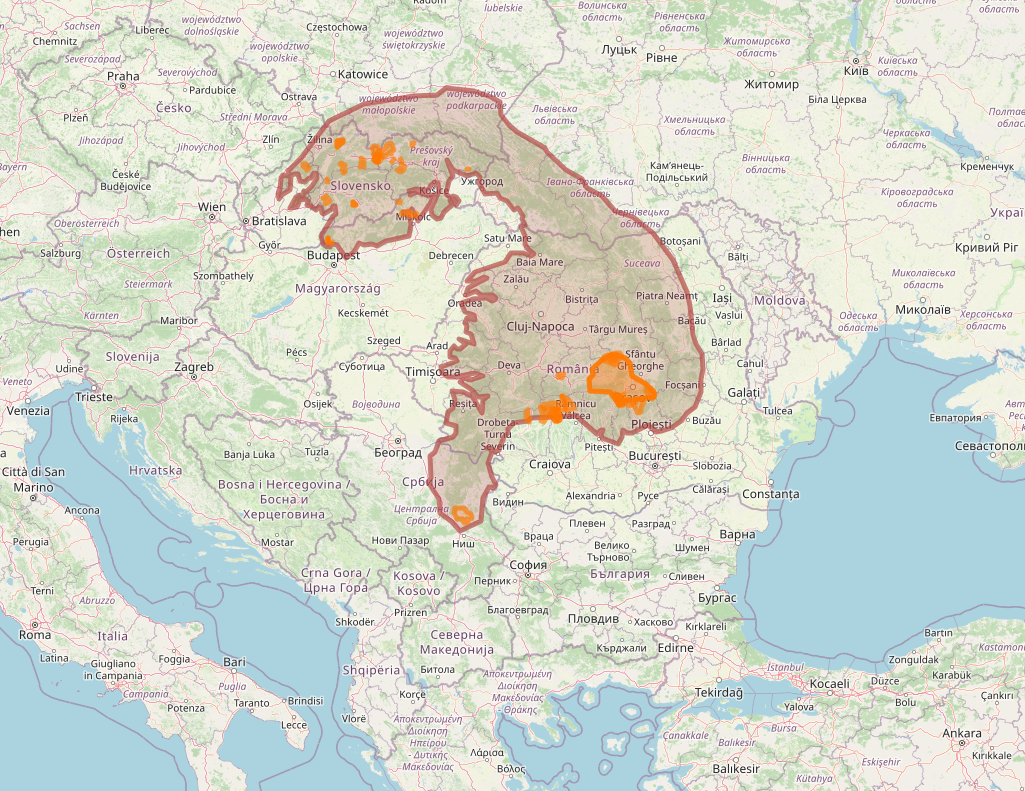
\includegraphics[scale=0.6]{img/carpathian.png}}
    \caption{Visualization of Q1}
    \label{fig:carpathian}
\end{figure}


\subsubsection*{Q2 - Value chains operating around Trento city (Italy)}
In the following, we report the GeoSPARQL query corresponding to Q2. The results are displayed in \Cref{fig:trento}.

\begin{lstlisting}[caption=GeoSPARQL Query 2, label={lst:query2}]
PREFIX /*!\gls{uom}!*/  <http://www.opengis.net/def/uom/OGC/1.0/>
PREFIX /*!\gls{rdfs}!*/  <http://www.w3.org/2000/01/rdf-schema#>
PREFIX /*!\gls{geof}!*/  <http://www.opengis.net/def/function/geosparql/> 
PREFIX /*!\gls{geo}!*/  <http://www.opengis.net/ont/geosparql#>
PREFIX /*!\gls{narra}!*/  <https://dlnarratives.eu/ontology#>
SELECT ?nlabel ?clabel ?wktLau
WHERE { 
       {
    ?narra narra:isAboutCountry ?country ;
            narra:isAboutLAU ?lau ;
            rdfs:label ?nlabel .
    ?country rdfs:label ?clabel .
    ?lau geo:hasGeometry ?glau .
    ?glau geo:asWKT ?wktLau .
}
    FILTER(geof:sfIntersects(
        ?wktLau,
        geof:buffer(
            "POINT(11.12108 46.06787)"^^geo:wktLiteral,
        0.5, uom:degree))). 
}
\end{lstlisting}

The \Cref{lst:query2} extracts the \acrshort{VCLabel}titles, countries and LAU geometries of the value chains operating within a maximum distance of 23 km from Trento. The query structure is similar to the one of Q1, with the difference that it does not use an external endpoint to retrieve the reference geometry. Instead, the FILTER clause operates an intersection between all \acrshortpl{VCLabel}' LAU geometries and a circular buffer of 0.3 degrees ($\sim$40 km) around the Trento longitude-latitude coordinates. 

The query produced the results visualised in \Cref{fig:trento}. As in the case of Q1, the expert's evaluation highlighted that the \acrshortpl{LAULabel} retrieved by this query were correct and complete (Precision and Recall were 1). Therefore, the query was valuable in retrieving city-specific \acrshortpl{VCLabel}.


\begin{figure}[h!tb]
    \centerline {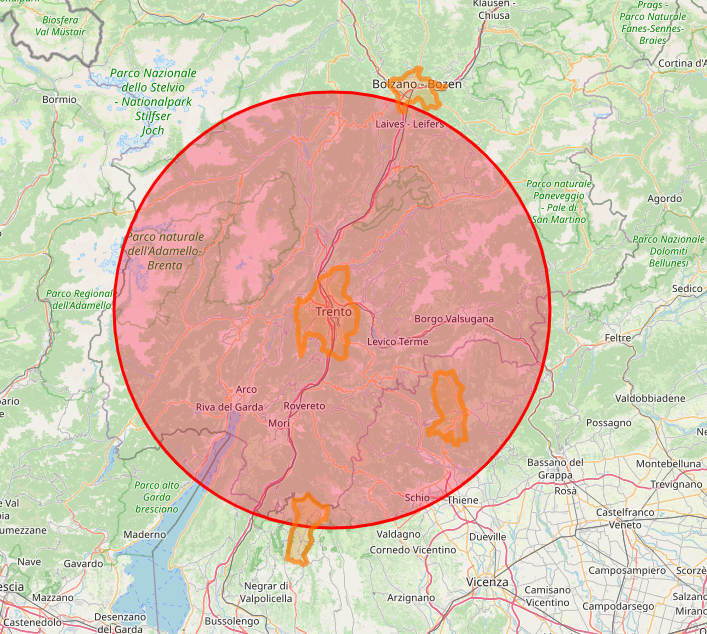
\includegraphics[scale=0.6]{img/trento.png}}
    \caption{Visualization of Q2}
    \label{fig:trento}
\end{figure}

\subsubsection*{Q3 - Value chains operating in Iberian Peninsula}
In the following, we report the GeoSPARQL query corresponding to Q3. The results are displayed in \Cref{fig:iberian}.

\begin{lstlisting}[caption=GeoSPARQL Query 3, label={lst:query3}]
PREFIX /*!\gls{uom}!*/ <http://www.opengis.net/def/uom/OGC/1.0/>
PREFIX /*!\gls{rdfs}!*/ <http://www.w3.org/2000/01/rdf-schema#>
PREFIX /*!\gls{geof}!*/ <http://www.opengis.net/def/function/geosparql/> 
PREFIX /*!\gls{geo}!*/ <http://www.opengis.net/ont/geosparql#>
PREFIX /*!\gls{narra}!*/ <https://dlnarratives.eu/ontology#>
PREFIX /*!\gls{osm}!*/ <https://www.openstreetmap.org/>
PREFIX /*!\gls{wd}!*/  <http://www.wikidata.org/entity/>
PREFIX /*!\gls{osm2rdfkey}!*/ <https://osm2rdf.cs.uni-freiburg.de/rdf/key#>

SELECT ?nlabel ?clabel ?wktLau 
WHERE  
    {   
        ?narra narra:isAboutCountry ?country ;
           narra:isAboutLAU ?lau ;
    	      rdfs:label ?nlabel .
    ?country rdfs:label ?clabel .
    ?lau geo:hasGeometry ?glau .
    ?glau geo:asWKT ?wktLau .
   { SELECT ?wkt WHERE {
        	SERVICE 
      		  <https://qlever.cs.uni-freiburg.de/api/osm-planet> { 
            	?osm_id osm2rdfkey:wikidata wd:Q12837 ;
                        a osm:relation ;
                        geo:hasGeometry ?geometry .
                ?geometry geo:asWKT ?wkt .
                
        	} 
    	} LIMIT 1
  	}
     FILTER(geof:sfWithin(?wktLau,?wkt)). 
}
\end{lstlisting}

The \Cref{lst:query3} extracts the \acrshort{VCLabel}titles, countries, and LAU geometries of the value chains operating in Scotland. The query structure is still similar to that of Q1. It uses the same external QLever Open Street Map endpoint to retrieve the geometry of Iberian Peninsula boundaries. The \texttt{FILTER} clause operates the intersection between Iberian Peninsula and the \acrshortpl{VCLabel}' LAU geometries. 

The query produced the results reported in \Cref{fig:iberian}. The expert's evaluation highlighted that the \acrshortpl{LAULabel} this query retrieved were correct and complete (Precision and Recall were 1). Therefore, the query was valuable in retrieving country-specific \acrshortpl{VCLabel}.


\begin{figure}[h!tb]
    \centerline {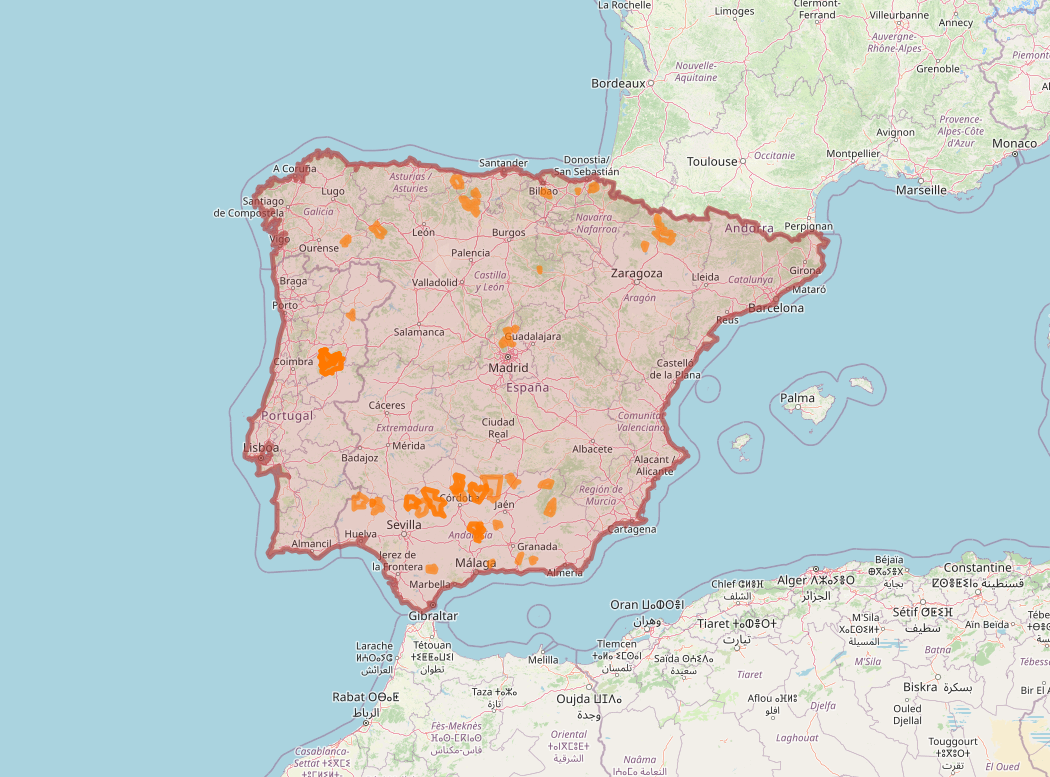
\includegraphics[scale=0.6]{img/iberian.png}}
    \caption{Visualization of Q3}
    \label{fig:iberian}
\end{figure}

\subsubsection{Q4 - Value chains operating around long European rivers}
In the following, we report the GeoSPARQL query corresponding to Q4. The results are displayed in \Cref{fig:rivers}.

\begin{lstlisting}[caption=GeoSPARQL Query 4, label={lst:query4}]
PREFIX /*!\gls{osmkey}!*/ <https://www.openstreetmap.org/wiki/Key:>
PREFIX /*!\gls{wd}!*/ <http://www.wikidata.org/entity/>
PREFIX /*!\gls{osm}!*/ <https://www.openstreetmap.org/>
PREFIX /*!\gls{wdt}!*/ <http://www.wikidata.org/prop/direct/>
PREFIX /*!\gls{uom}!*/ <http://www.opengis.net/def/uom/OGC/1.0/>
PREFIX /*!\gls{rdfs}!*/ <http://www.w3.org/2000/01/rdf-schema#>
PREFIX /*!\gls{geof}!*/ <http://www.opengis.net/def/function/geosparql/> 
PREFIX /*!\gls{geo}!*/ <http://www.opengis.net/ont/geosparql#>
PREFIX /*!\gls{narra}!*/ <https://dlnarratives.eu/ontology#>
PREFIX /*!\gls{osm2rdfkey}!*/ <https://osm2rdf.cs.uni-freiburg.de/rdf/key#>

SELECT ?nlabel ?clabel ?wktLau 
WHERE { 
    ?narra narra:isAboutCountry ?country ;
            narra:isAboutLAU ?lau ;
            rdfs:label ?nlabel .
    ?country rdfs:label ?clabel .
    ?lau geo:hasGeometry ?glau .
    ?glau geo:asWKT ?wktLau .
{
SELECT DISTINCT ?river_osm ?river_wd ?river_name ?length ?wkt WHERE {
    SERVICE <https://qlever.cs.uni-freiburg.de/api/osm-planet> {
        ?river_osm a osm:relation ;
                osmkey:waterway ?waterway ;
                geo:hasGeometry ?geometry ;
                osmkey:name ?river_name ;
                osm2rdfkey:wikidata ?river_wd .
        ?geometry geo:asWKT ?wkt .
    SERVICE <https://qlever.cs.uni-freiburg.de/api/wikidata> {
        ?river_wd wdt:P31/wdt:P279* wd:Q4022 ;
                wdt:P30 wd:Q46 ;
                wdt:P2043 ?length .
        FILTER (?length > 500)
    }
    }
} ORDER BY DESC(?length) 
}
FILTER(geof:sfIntersects(?wktLau, ?wkt)). 
}

\end{lstlisting}

The \Cref{lst:query4} retrieves all \acrshortpl{VCLabel} operating close to a European river longer than 500 km. The query structure is very similar to that of Q1 and uses the same external endpoint. The main differences are the following:
\begin{itemize}
    \item the nested \texttt{SELECT} clause operates on two different QLever-instance subgraphs: Open Street Map and Wikidata. The query retrieves the river geometries from the first. Then it uses the second to retrieve the list of "rivers" (\gls{wd}Q4022) present in "Italy" (\gls{wd}Q46) whose "length" (id. P2043) exceeds 500km ("FILTER (?length > 500)"); 
    \item the final \texttt{FILTER} clause operates the intersection between the Italian rivers and the \acrshortpl{VCLabel}' LAU geometries. 
\end{itemize}

The query produced the results reported in \Cref{fig:rivers}. All \acrshortpl{VCLabel} retrieved were correct and complete (Precision and Recall were 1). Therefore, the query was valuable in retrieving river-related \acrshortpl{VCLabel} and, by extension, could be used to extract water-basin-related \acrshortpl{VCLabel}.

\begin{figure}[h!tb]
    \centerline {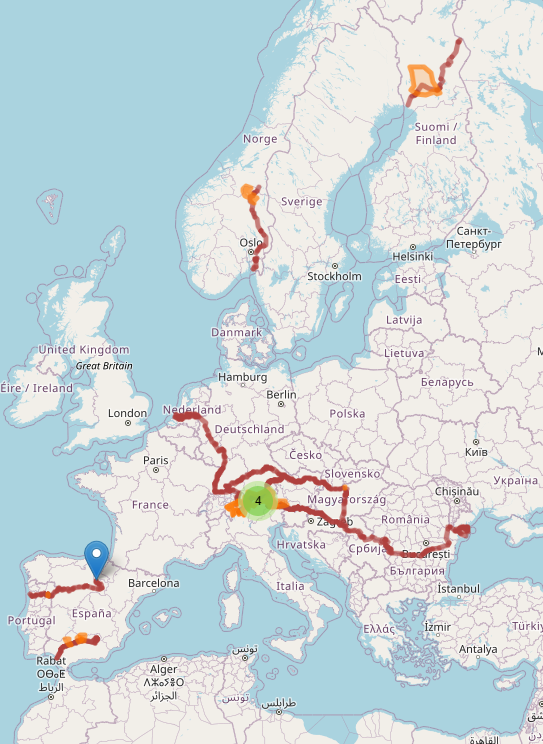
\includegraphics[scale=0.6]{img/rivers.png}}
    \caption{Visualization of Q4}
    \label{fig:rivers}
\end{figure}


\subsection{Visualization: Story Maps}\label{VII-subsec:moving-visualization}

Story maps are tools for visualizing narratives by embedding story events in spatial contexts. To visualize the 454 VC, we used a module of the Storymaps Building and Visualizing Tool (SMBVT) \cite{bartalesiWebToolCreate2023b}, which allows narratives to be mapped interactively, enhancing user engagement and understanding through multimedia and spatial linking. SMBVT employs Storymap.js \cite{zhaoJakobzhaoStorymap2024}, a JavaScript library for creating interactive map-based stories, which has been customized to meet the specific needs of SMBVT’s narrative visualization. Moreover, this visualization technique directly addresses Research Question 3 (\ref{quote:rq3}), demonstrating its efficacy in enhancing the interpretability and accessibility of complex narrative data through geospatial representation.

\begin{figure*}[h!tb]
\begin{multicols}{2}
    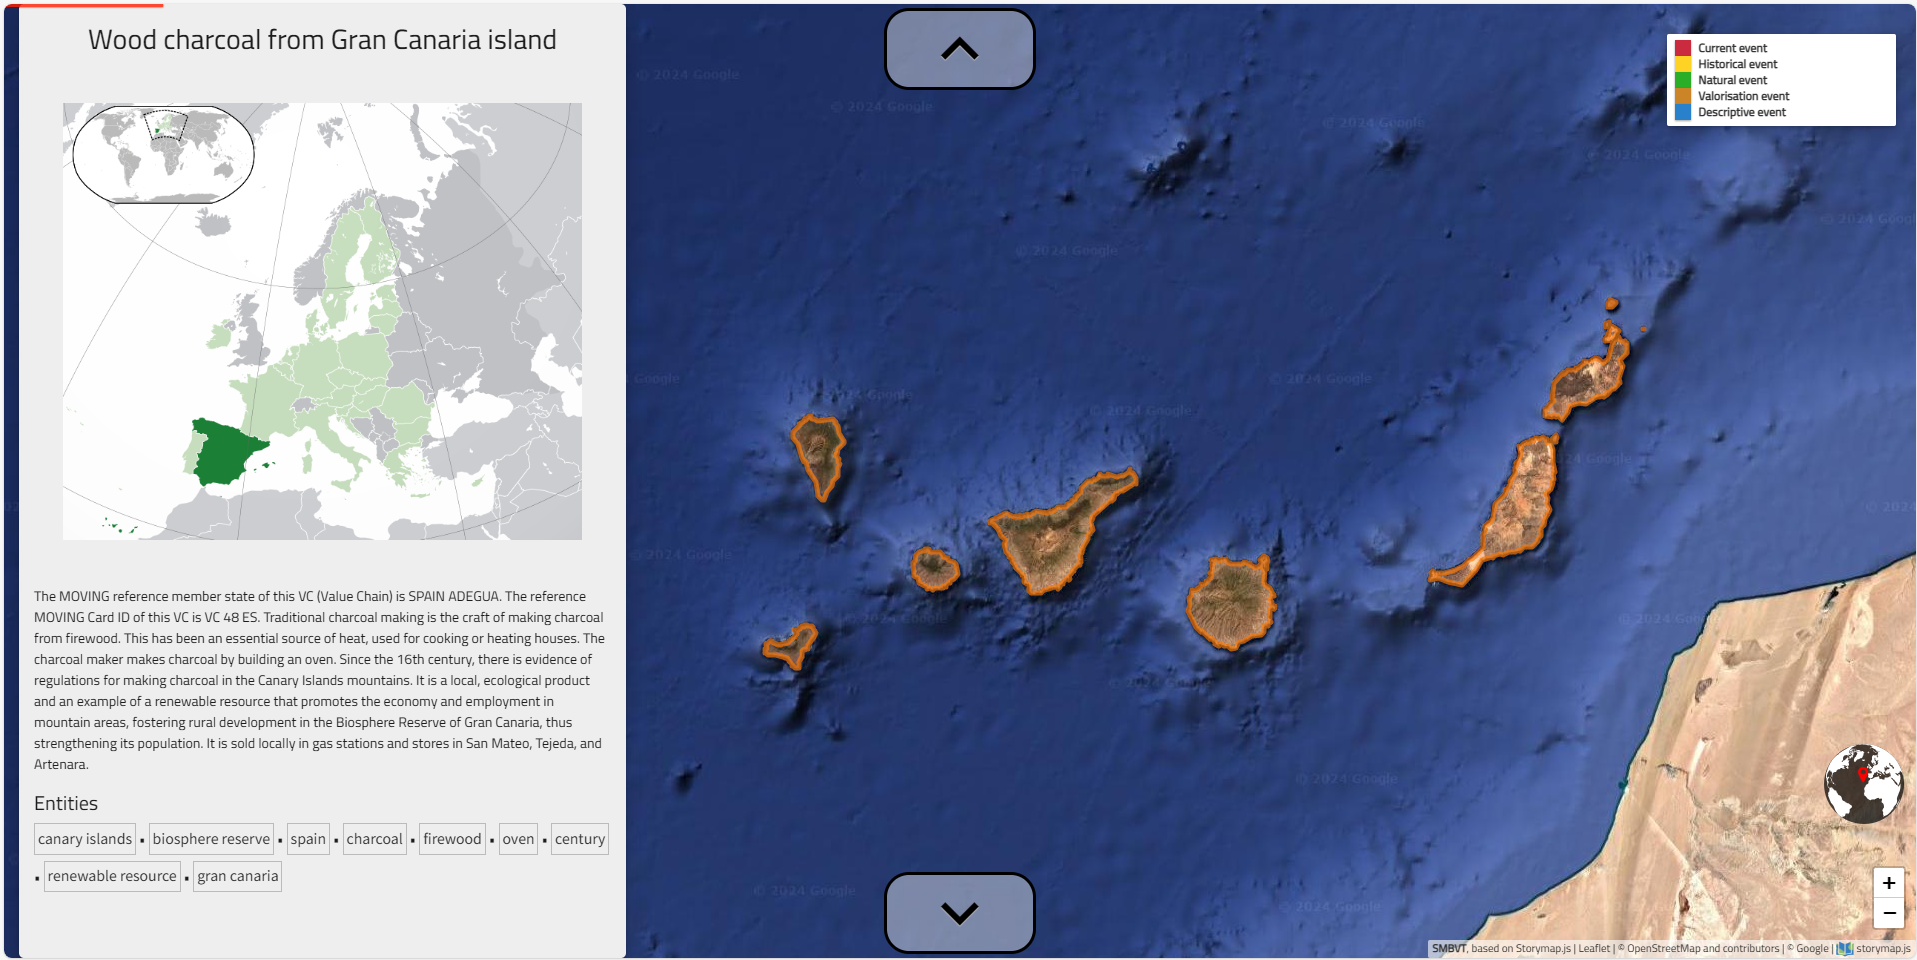
\includegraphics[width=\linewidth]{img/charcoal1.png}
    \caption{Caption here}\label{fig:charcoal1}\par 
    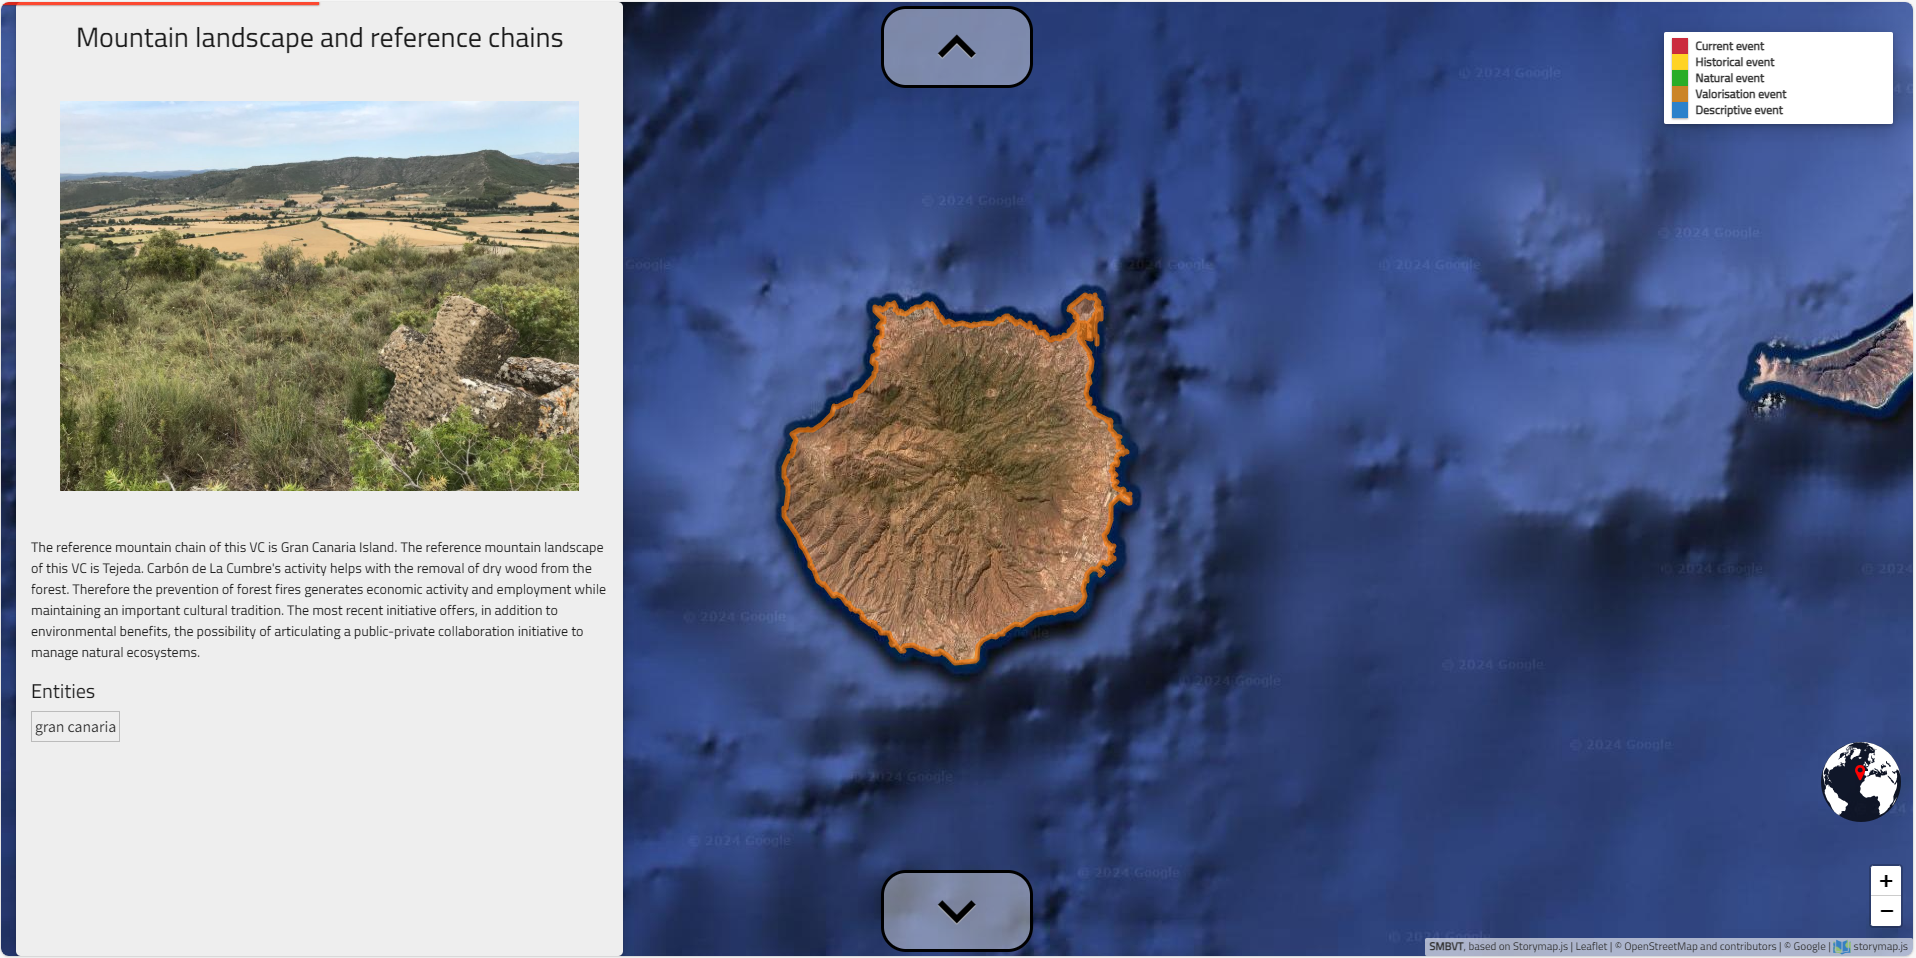
\includegraphics[width=\linewidth]{img/charcoal2.png}
    \caption{Caption here}\label{fig:charcoal2}\par 
\end{multicols}
\begin{multicols}{2}
    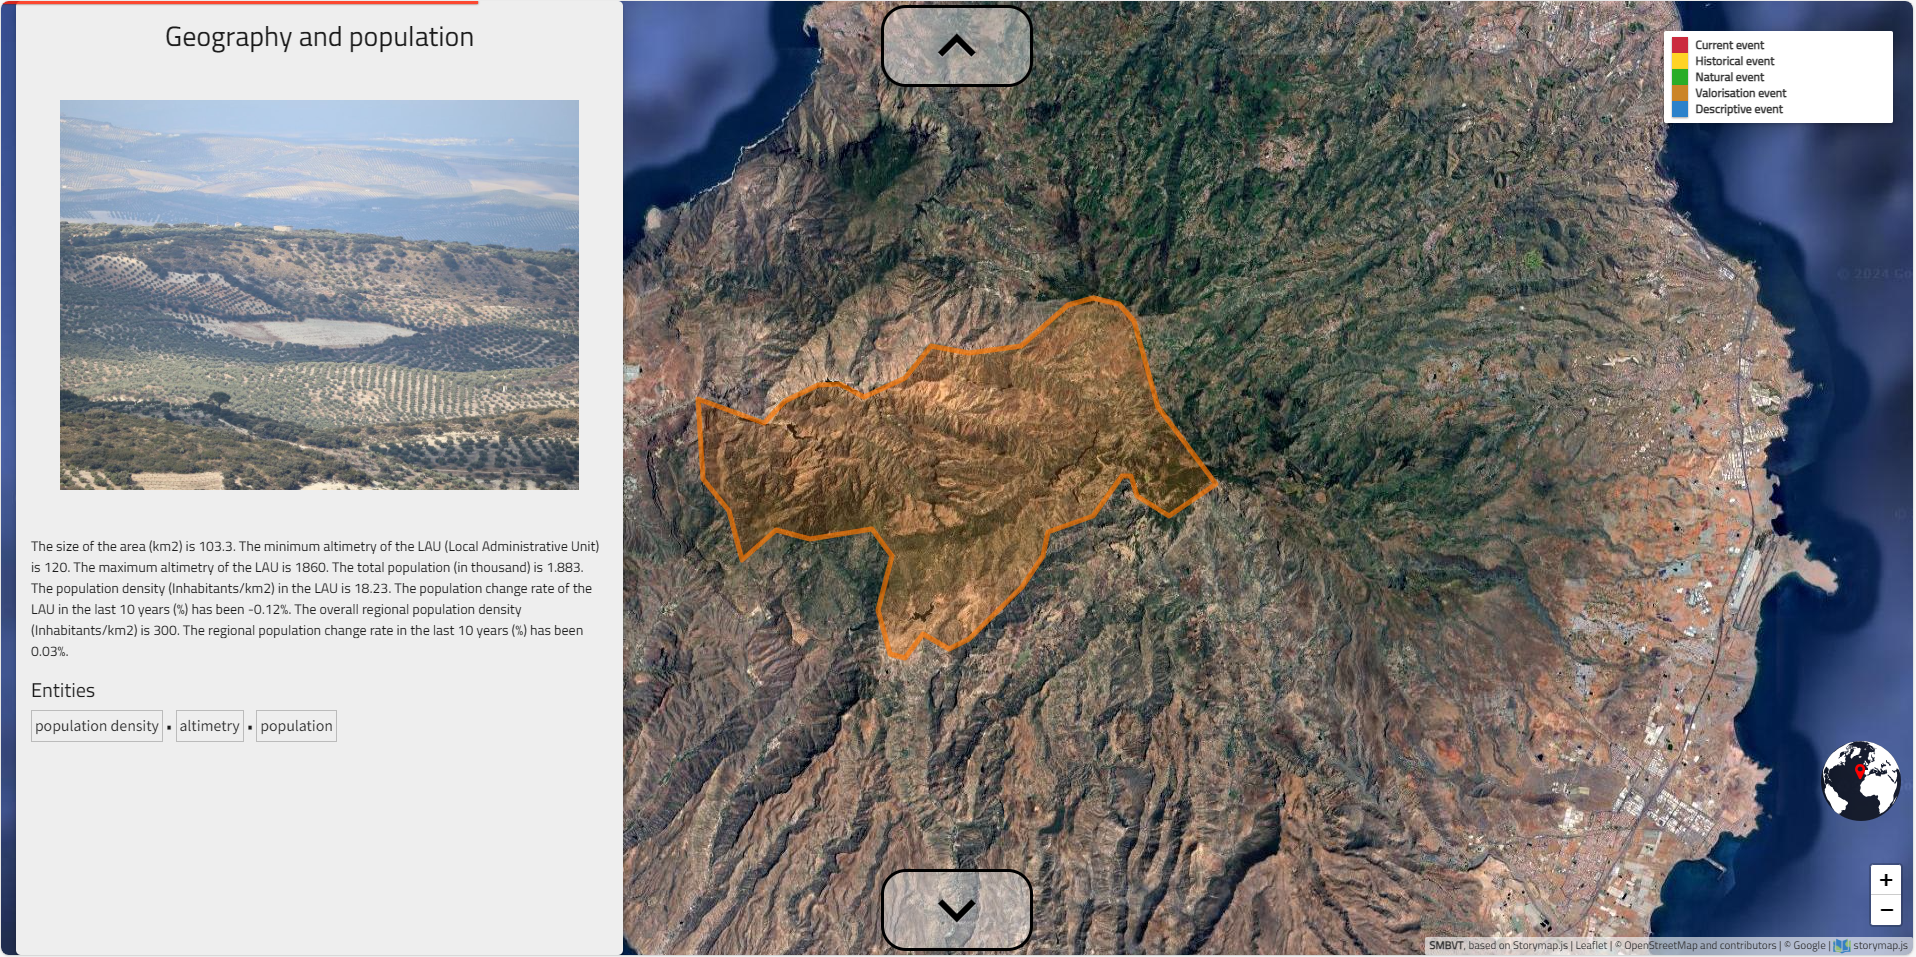
\includegraphics[width=\linewidth]{img/charcoal3.png}
    \caption{Caption here}\label{fig:charcoal3}\par
    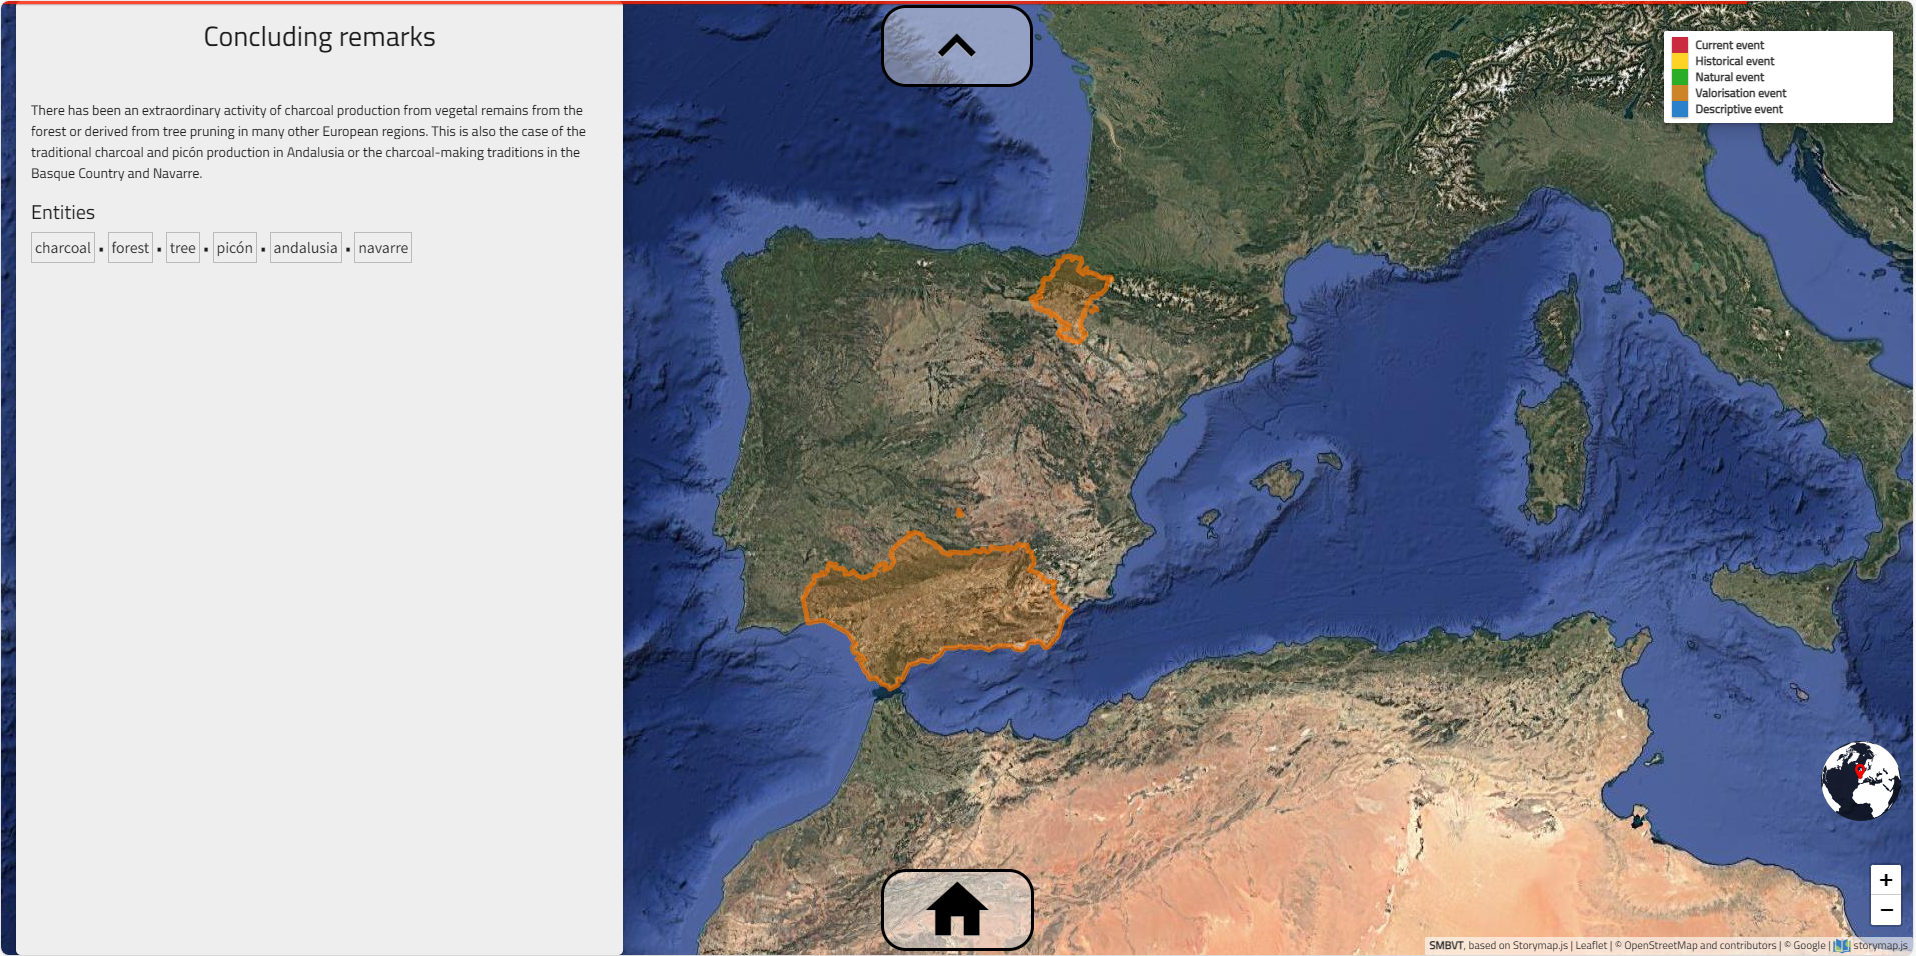
\includegraphics[width=\linewidth]{img/charcoal4.png}
    \caption{Caption here}\label{fig:charcoal4}\par
\end{multicols}
\end{figure*}

\subsubsection{Components of SMBVT Story Maps}
In SMBVT, a story map comprises several interactive components that guide the user through the narrative in a plot-defined sequence. Each story event is represented on the map as a distinct “slide,” containing essential information that enhances the storytelling experience. Each event on the story map is associated with:

\begin{itemize}
    \item \textbf{Geographic Location}: Geographic coordinates or polygons are displayed on the map, providing spatial context (\Cref{fig:charcoal1,fig:charcoal2,fig:charcoal3,fig:charcoal4}).
    \item \textbf{Media Objects}: An image or video linked to each event, known as the "media object", serves as a preview and provides visual engagement (\Cref{fig:charcoal1,fig:charcoal2,fig:charcoal3}).
    \item \textbf{Descriptive Text}: A title and narrative description enrich each event’s context (\Cref{fig:charcoal1,fig:charcoal2,fig:charcoal3,fig:charcoal4}).
    \item \textbf{Entities}: Links to external sources, including Wikidata entities and digital objects on platforms like Europeana, facilitate deeper exploration (\Cref{fig:charcoal1,fig:charcoal2,fig:charcoal3,fig:charcoal4}).
\end{itemize}

There are two arrows, one at the center top of the page and the other at the bottom, allowing navigation through the slides. The last slide (\Cref{fig:charcoal4}) has a home icon to return to the first slide.

Each slide on the story map is divided into two parts:
\begin{itemize}
    \item \textbf{Background Map}: Displayed on the right side, the background map shows the geographical elements.
    \item \textbf{Event Information}: Displayed on the left side, this section provides detailed information about each event, including media objects and descriptive text.
\end{itemize}

Storymap.js was selected for its flexibility in handling large background maps and supporting data represented as JSON. Its slide-based approach to storytelling aligns well with SMBVT’s narrative structure, where each event is encapsulated in a slide that combines spatial and informational elements.

\begin{figure}[h!tb]
    \centerline {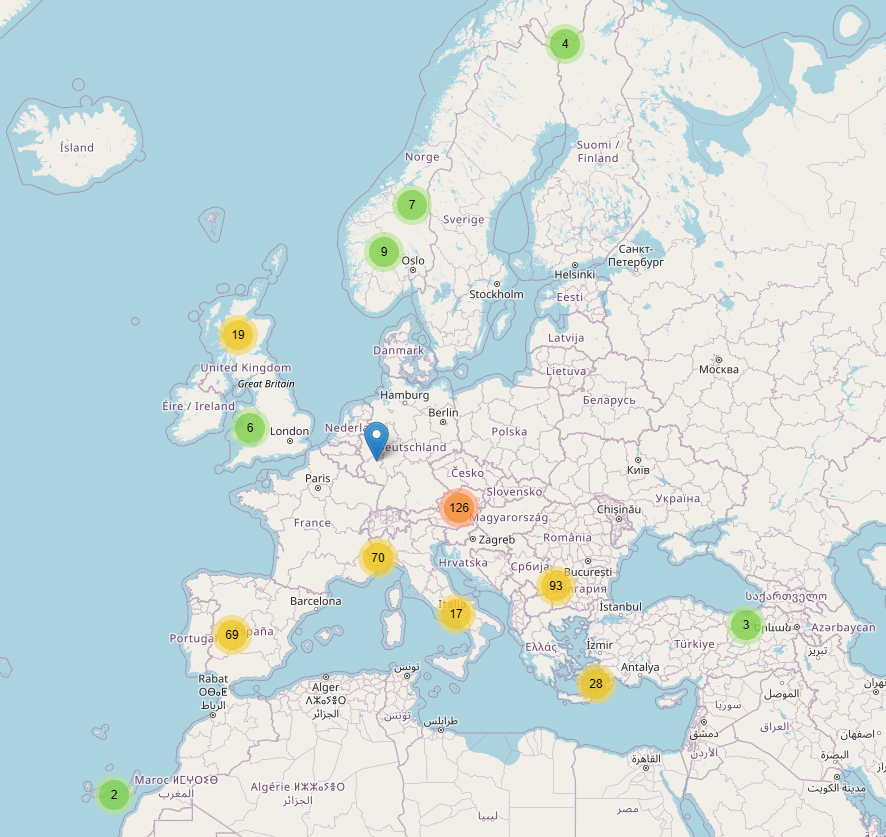
\includegraphics[scale=0.6]{img/allStorymapsMoving.png}}
    \caption{All 454 Story Maps on the map}
    \label{fig:allStorymaps}
\end{figure}

All story maps can be accessed through a map interface that allows users to explore an additional geospatial dimension, connecting each story with others in spatial relation (\Cref{fig:allStorymaps}).

\subsubsection{Publication and Static Web Application Generation}
Once a story map is fully compiled, SMBVT generates a static Web application. This Web app encapsulates all necessary JSON data, JavaScript functionality, and external libraries, creating an interactive experience for end users. The final output enables users to explore the narrative through a series of map-based events, fully contained within a single Web application.

SMBVT’s story maps, facilitated by the customization of StoryMapJS, offer a dynamic and immersive way to present narratives within a spatial context. This tool’s flexibility and ease of integration make it highly effective for storytelling in digital and educational applications, connecting users with content interactively and meaningfully.


\section{Medioeval and Reinassence Geographic Literature (IMAGO Project 2020-2024)}\label{VII-sec:imago}

The \acrfull{IMAGOLabel} project \cite{IMAGOProject} is dedicated to the study of medieval and Renaissance geographical works, ranging from the 6th to the 15th centuries. This interdisciplinary project aims to provide a comprehensive survey of geographic works, classifying authors, genres, and contents, while also collecting manuscripts, editions, and bibliographies of these works. 

\acrshort{IMAGOLabel} focuses on building a web portal and a knowledge base (KB) to facilitate research in medieval geography by using Semantic Web technologies. 

For the \acrshort{IMAGOLabel} project, the dataset focused on geospatial data found in historical texts, particularly locations cited in medieval manuscripts. The second module of the algorithm was instrumental in enriching this dataset, as it incorporated geospatial information from \acrshort{OSMLabel} and linked these places to relevant Wikidata entities.

Using the NOnt+S ontology framework, I developed a knowledge base to represent geospatial knowledge within historical geographic texts. The application of semantic reasoning to this dataset revealed connections between geographic references across various historical texts, providing new insights into medieval geography. The ontology was also used to model the structure of medieval travel narratives, preserving the historical context of these journeys. This approach facilitated the analysis and comparison of different medieval travel routes, cultural exchanges, and traveler experiences, enhancing our understanding of historical travel patterns.

\subsection{Linking and Geospatial Enrichment}\label{VII-subsec:imago-linking}

In the annotation of medieval and Renaissance geographical texts, scholars employed a semi-automatic tool designed to capture and document extensive bibliographic details. These details encompassed not only the geographical texts themselves but also the manuscripts and printed editions through which these texts have been transmitted. Given the inherently geographical nature of these works, the annotations were enriched with a comprehensive set of geospatial data. This data spanned a wide range of entities, including the geographic locations mentioned within the texts, as well as the present-day locations of the libraries and archives that held these manuscripts and print editions.

The geospatial information collected from these texts was significantly enhanced by linking it to a variety of geospatial knowledge bases. The historical dimension of these works posed a unique challenge: many of the geographical places referenced either no longer exist or have undergone substantial transformation across the centuries. Addressing this challenge required linking the annotated geospatial data not only to contemporary databases but also to specialized historical knowledge repositories. One such critical resource was Pleiades \cite{simonPleiadesGazetteerPelagios2016}, a robust and authoritative knowledge base dedicated to ancient geographic locations. The integration with Pleiades enabled scholars to situate historical places accurately within their appropriate temporal and cultural contexts, facilitating a more nuanced understanding of these geographic references. This phase of linking was, therefore, pivotal in establishing a reliable and contextually aware framework for the spatial data embedded within the medieval and Renaissance texts.

The \acrshort{IMAGOLabel} knowledge base, structured using the same foundational ontologies as the NOnt framework, the CRM and the LRMoo, facilitates seamless interoperability between these two knowledge systems. This common ontological foundation permits the merging of both knowledge bases, ensuring that data exchange and integration processes are both efficient and semantically coherent. The structural compatibility between \acrshort{IMAGOLabel} and NOnt+S thus allows for enhanced information retrieval and more sophisticated knowledge representation.

Subsequent to the linking phase, a comprehensive geospatial enrichment phase was undertaken. This phase utilized the \Cref{alg:entityextraction}, a module explicitly developed to support advanced querying of linked data sources. Through the execution of these queries, the scholars were able to extract additional geospatial details from widely used and openly accessible datasets such as \acrshort{OSMLabel} and Wikidata. These datasets offered a rich repository of information, including precise coordinates and polygonal representations of various geographical features. By incorporating this enriched data, the scholars were able to augment the initial annotations, providing a more detailed and accurate spatial representation of the places referenced in the texts.

This enrichment process not only increased the depth of the annotated geospatial data but also enabled the visualization and mapping of historical locations described in the medieval and Renaissance texts. Such visualizations afford new insights into the spatial dynamics of the works, illuminating the complex geographical relationships that shaped the understanding of space and place in these historical periods. Consequently, the enriched geospatial framework contributes to a more profound and comprehensive exploration of the historical and cultural landscapes depicted in these texts.


\subsection{Knowledge Graph Creation and Storage}\label{VII-subsec:imago-kg}

The \acrshort{IMAGOLabel} knowledge graph\footnote{The graph can be downloaded at \url{https://geosparql.isti.cnr.it/ontology/imago.owl}} was constructed in accordance with the comprehensive framework outlined in  \Cref{chap:SW-framework}. This framework provided a systematic approach, ensuring that each stage of knowledge graph development adhered to the principles of semantic web technologies, data interoperability, and ontological consistency. The creation process involved a design phase, wherein concepts and relationships relevant to the domain of medieval and Renaissance geographical works were modeled using well-established ontologies, particularly the CIDOC Conceptual Reference Model (CRM) and the Library Reference Model object-oriented version (LRMoo). These ontologies served as the foundational schema, ensuring semantic clarity and facilitating seamless integration with other linked datasets.

A key consideration during the development of the \acrshort{IMAGOLabel} knowledge graph was the need to accommodate the rich geospatial information inherent in the annotated works. To this end, the graph was structured to support complex geospatial queries, a requirement that was addressed through the integration of GeoSPARQL. GeoSPARQL, an extension of the SPARQL query language specifically designed for geospatial data, provided the necessary tools to handle the intricate spatial relationships and geometries associated with the geographical references in the texts. By leveraging GeoSPARQL, the knowledge graph not only enabled efficient querying of spatial data but also supported advanced geospatial operations, such as the retrieval of location-based information and the computation of spatial relationships.

The storage of the \acrshort{IMAGOLabel} knowledge graph was implemented using a Fuseki triplestore, a robust and scalable RDF (Resource Description Framework) database solution optimized for handling linked data. Fuseki’s compatibility with GeoSPARQL allowed for the seamless storage and retrieval of geospatial data, ensuring that the knowledge graph remained performant and responsive to complex queries. Furthermore, the use of a triplestore architecture ensured that the data remained flexible and easily extendable, accommodating future updates and integrations with minimal disruption.

By employing these technologies, the \acrshort{IMAGOLabel} knowledge graph became a powerful tool for exploring and analyzing the intricate web of relationships between historical texts, places, and cultural heritage objects. The combination of semantic precision, geospatial enrichment, and efficient data storage ensured that the graph could be used effectively by scholars and researchers to gain new insights into the spatial and temporal dimensions of medieval and Renaissance geography. Thus, the creation and storage strategy of the \acrshort{IMAGOLabel} knowledge graph exemplified a sophisticated approach to knowledge representation, grounded in the principles of the semantic web and designed to support both scholarly inquiry and digital heritage preservation.


\subsection{Consistency of the Knowledge Graph}\label{VII-subsec:imago-consistency}

To check the consistency of the knowledge graph is employed Openllet\cite{galigatorGaligatorOpenllet2024} as described in the \Cref{chap:SW-framework}. These tools analyze the graph for logical inconsistencies, such as contradictory relationships or incorrect classifications. For instance, if a geographic work is incorrectly linked to a location that did not exist during the time period in question, the reasoning engine can flag this as an inconsistency.

Another important aspect of maintaining consistency is ensuring the proper integration of external data sources. Linked Data often involves incorporating information from various knowledge bases, each of which may use slightly different ontological models. Alignment of these models through ontology matching and mapping techniques ensures that the data remains semantically coherent across sources.

Regular consistency checks are also necessary as the knowledge graph evolves. As new data is added or existing data is updated, automatic or semi-automatic validation mechanisms must be in place to ensure that the graph remains logically sound and free from errors.

\subsection{Requirement Analysis and Querying}\label{VII-subsec:imago-querying}

Before effective querying of the knowledge graph can take place, a thorough requirement analysis must be conducted. This involves identifying the key research questions that the knowledge graph is intended to address, as well as the specific types of information that users will need to retrieve. Requirement analysis serves as the foundation for designing efficient GeoSPARQL queries and ensuring that the structure of the knowledge graph supports the desired use cases.

During the requirement analysis phase, scholars and domain experts collaborate to outline the types of queries they anticipate running against the knowledge graph. These could include retrieving all works that reference a particular geographic location, finding all manuscripts stored in a specific archive, or identifying the spatial relationships between different historical places. The specific needs of the user community must be thoroughly understood so that the data model, ontologies, and graph structure are optimized for these queries.

Once the requirements are clearly defined, the next step is to create GeoSPARQL queries that can extract the relevant data. GeoSPARQL is a powerful query language specifically designed for querying \acrshort{RDFLabel} datasets. Its pattern-matching capabilities enable users to express complex queries involving multiple entities and relationships. For instance, a query could retrieve all places mentioned in a set of geographical works, along with their modern equivalents retrieved from external geospatial knowledge bases such as \acrshort{OSMLabel}.

Query optimization is another important consideration during this phase. As knowledge graphs grow in size and complexity, performance can become an issue. Therefore, the design of \acrshort{SPARQLLabel} queries must account for factors such as execution time, memory usage, and indexing. Efficient query design ensures that the knowledge graph remains responsive and usable, even as the amount of data increases. Additionally, designing and executing a distinct set of queries in this domain, separate from those outlined in Section \ref{VII-subsec:moving-querying}, is essential to reinforce the robustness of responses to Research Question 2 (\ref{quote:rq2}). This approach not only validates the applicability of the methodology across diverse contexts but also underscores the adaptability and scalability of the proposed query framework.


We focussed on four types of knowledge-extraction targets, corresponding to four GeoSPARQL queries regarding different and complementary aspects of medieval manuscripts and their related place cited:
\begin{enumerate}
    \item The works that mention places located in France (Q5)
    \item The places located within a 0.2-degree buffer around the Via Francigena (Q6)
    \item The places in Italy that are mentioned in works contained in manuscripts written in the fifteenth century (Q7)
    \item The authors who have visited the Holy Land (Q8)
\end{enumerate}

The information extracted by these queries covered the interests of the \acrshort{IMAGOLabel} scholars. It would have been hard, indeed, to extract the same information through the usual data representation and technology adopted by this community. Based on the query results\footnote{The visualization of the queries can be replicated via the web application accessible at \url{https://github.com/prate91/GeoSPARQL-queries-visualization-for-thesis}}, we calculated the same standard performance of \Cref{VII-subsec:moving-querying}. 

Even for \acrshort{IMAGOLabel} queries, the performance metrics displayed in \Cref{tab:evaluationQueries} uniformly indicate a perfect score of 1 for Precision, Recall, and F1. This consistency across diverse queries further corroborates the comprehensive reliability and robustness of our knowledge graph. The ability to maintain such high performance across various query scenarios reflects the effectiveness of the semantic structures and inference mechanisms we have implemented. These results underscore the high fidelity and precision of our data representation, which facilitates accurate and exhaustive retrieval, thereby enhancing the utility and reliability of our system. In the following, we report the details of the queries and the corresponding results.

\begin{table}[H]
    \centering
        \caption{Precision, Recall, and F1 measurements of IMAGO queries.}
    \label{tab:evaluationQueriesIMAGO}
    \begin{tabular}{|l|l|l|l|}
    \hline
 Query & Precision & Recall & F1\\
\hline
        Q5 & 1 & 1 & 1\\ \hline
        Q6 & 1 & 1 & 1\\ \hline
        Q7 & 1 & 1 & 1 \\  \hline
        Q8 & 1 & 1 & 1 \\ \hline
    \end{tabular}
\end{table}

\subsubsection*{Q5 - The works that mention places located in France}
In the following, we report the GeoSPARQL query corresponding to Q5. The results are displayed in \Cref{fig:france}.

\begin{lstlisting}[caption=GeoSPARQL Query 5, label={lst:query5}]
PREFIX /*!\gls{imago}!*/ <https://imagoarchive.it/ontology/>
PREFIX /*!\gls{wd}!*/ <http://www.wikidata.org/entity/>
PREFIX /*!\gls{geo}!*/ <http://www.opengis.net/ont/geosparql#>
PREFIX /*!\gls{ecrm}!*/ <http://erlangen-crm.org/200717/>
PREFIX /*!\gls{ilrm}!*/ <http://imagoarchive.it/ilrmoo/>
PREFIX /*!\gls{osm}!*/ <https://www.openstreetmap.org/>
PREFIX /*!\gls{osm2rdfkey}!*/ <https://osm2rdf.cs.uni-freiburg.de/rdf/key#>
PREFIX /*!\gls{geof}!*/ <http://www.opengis.net/def/function/geosparql/> 

SELECT DISTINCT ?title ?authorName ?toponymName ?wktPlace
  FROM <https://geosparql.isti.cnr.it/fuseki/imago/archive>
WHERE {
  ?exp_cre a ilrm:F28_Expression_Creation ;
  	         ilrm:R17_created ?work ;
  	         ecrm:P14_carried_out_by ?author .	
  ?author a imago:Author ;
          ecrm:P1_is_identified_by/ecrm:P190_has_symbolic_content ?authorName .
  ?work a ilrm:F2_Expression ;
        ecrm:P102_has_title/ecrm:P190_has_symbolic_content ?title ;
        ecrm:P106_is_composed_of ?toponym .
  ?place imago:is_identified_by_toponym ?toponym ;
         geo:asWKT ?wktPlace .
  ?toponym ecrm:P190_has_symbolic_content ?toponymName .

  { 
    SELECT ?wktFrance 
    WHERE {
        SERVICE <https://qlever.cs.uni-freiburg.de/api/osm-planet> { 
            ?osm_id osm2rdfkey:wikidata wd:Q142 ;
                    a osm:relation ;
                    geo:hasGeometry ?geometryFrance .
            ?geometryFrance geo:asWKT ?wktFrance .     
        } 
    } LIMIT 1
  }
  FILTER(geof:sfWithin(?wktPlace,?wktFrance)). 
} 
\end{lstlisting}

% The query retrieves the work titles and authors along with the toponyms the works mention. The WHERE clause contains the conditions that need to be satisfied for each result. It involves several semantic-triple patterns connected by the "." or ";" operators. In this clause, we retrieve the work titles, authors, toponyms, and the polygons of the places identified by the toponyms. A nested SELECT statement allows retrieving the WKT geometry of France (Q142) from the QLever \acrshort{SPARQLLabel} server of the University of Freiburg. Finally, the FILTER clause selects the places included within the France polygon.


The \Cref{lst:query5} is designed to retrieve distinct titles of works, author names, place names (toponyms), and the \acrshort{WKTLabel} representation of place geometries within France. The purpose of this query is to locate specific works within the \acrshort{IMAGOLabel} archive, ensuring that the places mentioned are geographically located within the boundaries of France. The query performs a spatial relationship check to filter only those places that fall within France’s geographical borders.

The query starts by defining various prefixes (lines 1-8) that are essential for interpreting and utilizing the data from different ontologies. 

The \texttt{SELECT DISTINCT} statement (line 10) specifies the output variables:
\begin{itemize}
    \item \texttt{?title} - Title of the work.
    \item \texttt{?authorName} - Name of the author of the work.
    \item \texttt{?toponymName} - Name of the place (toponym).
    \item \texttt{?wktPlace} - \acrshort{WKTLabel}representation of the place's geometry.
\end{itemize}

The \texttt{FROM} clause (line 11) indicates the source graph:\\
\texttt{https://geosparql.isti.cnr.it/fuseki/imago/archive}.

The main \texttt{WHERE} block (lines 12-27) contains the conditions that define the data to be retrieved. It is divided into several graph patterns:

\textbf{Graph Patterns for Expression Creation and Author}
\begin{itemize}
    \item The triple pattern at line 13, \texttt{?exp\_cre a \gls{ilrm}F28\_Expression\_Creation}, identifies instances of expression creation events.
    \item The pattern \texttt{\gls{ilrm}R17\_created ?work} links these events to the created works.
    \item The triple pattern \texttt{\gls{ecrm}P14\_carried\_out\_by ?author} identifies the author responsible for the creation.
\end{itemize}

\textbf{Graph Patterns for Author Details}
\begin{itemize}
    \item \texttt{?author a imago:Author} ensures that the \texttt{?author} variable is of the type \textit{Author}.
    \item The \texttt{\gls{ecrm}P1\_is\_identified\_by/\gls{ecrm}P190\_has\_symbolic\_content ?authorName} pattern retrieves the author’s name.
\end{itemize}

\textbf{Graph Patterns for Work and Title}
\begin{itemize}
    \item \texttt{?work a \gls{ilrm}F2\_Expression} identifies works as instances of the \\ \texttt{F2\_Expression} class.
    \item \texttt{\gls{ecrm}P102\_has\_title/\gls{ecrm}P190\_has\_symbolic\_content ?title} retrieves the title of each work.
    \item \texttt{\gls{ecrm}P106\_is\_composed\_of ?toponym} links the work to toponyms (place names) associated with it.
\end{itemize}

\textbf{Graph Patterns for Place Geometry}
\begin{itemize}
    \item \texttt{?place \gls{imago}is\_identified\_by\_toponym ?toponym} connects a place with its toponym.
    \item \texttt{\gls{geo}asWKT ?wktPlace} retrieves the \acrshort{WKTLabel} geometry of the place.
    \item \texttt{?toponym \gls{ecrm}P190\_has\_symbolic\_content ?toponymName} retrieves the symbolic content (name) of the toponym.
\end{itemize}

\textbf{Nested SELECT Clause}
A nested \texttt{SELECT} block (lines 20-27) retrieves the \acrshort{WKTLabel} geometry of France. The details are as follows:
\begin{itemize}
    \item \textbf{SERVICE Clause}: The \texttt{SERVICE} keyword (line 22) is used to access the external QLever endpoint \url{https://qlever.cs.uni-freiburg.de/api/osm-planet}.
    \item The triple pattern \texttt{?osm\_id \gls{osm2rdfkey}wikidata \gls{wd}Q142} (line 23) retrieves the \acrshort{OSMLabel} relation that corresponds to the Wikidata entity for France (\gls{wd}Q142).
    \item \texttt{geo:hasGeometry ?geometryFrance} retrieves the geometry of France.
    \item \texttt{geo:asWKT ?wktFrance} provides the \acrshort{WKTLabel} representation of this geometry.
    \item The \texttt{LIMIT 1} clause restricts the results to a single instance.
\end{itemize}

\textbf{Spatial Filter}
The \texttt{FILTER} clause (line 28) uses the \texttt{\gls{geof}sfWithin} function to check if the place geometry (\texttt{?wktPlace}) is spatially within the geometry of France (\texttt{?wktFrance}). This ensures that only places within France are considered in the results.

\begin{figure}[h!tb]
    \centerline {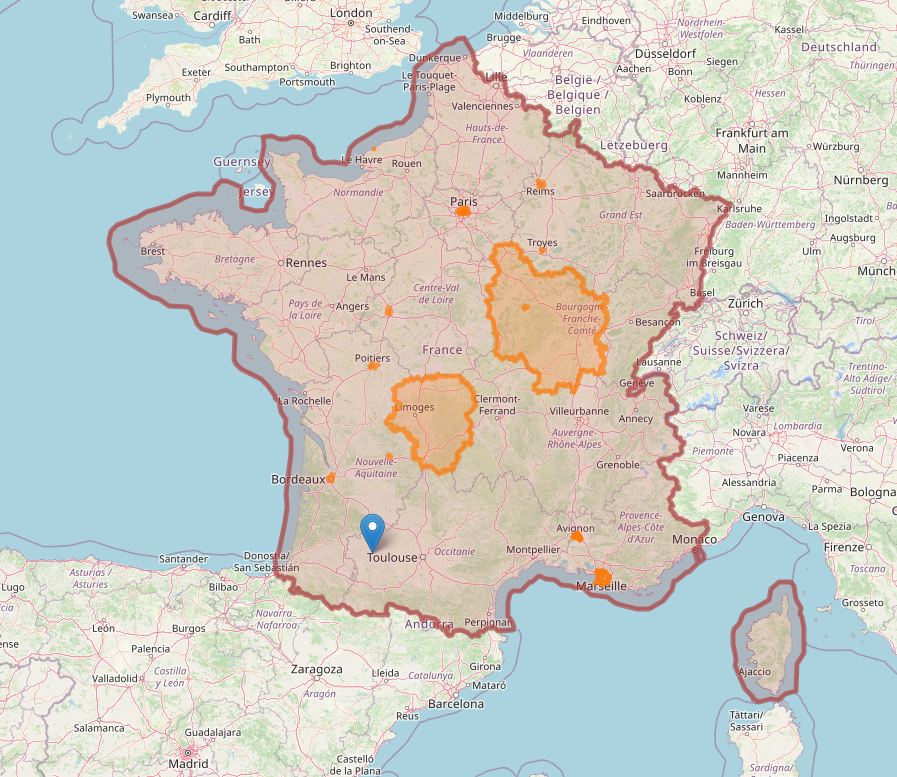
\includegraphics[scale=0.6]{img/france.png}}
    \caption{Visualization of Q5}
    \label{fig:france}
\end{figure}


\subsubsection*{Q6 - The places located within a 0.2-degree buffer around the Via Francigena}
In the following, we report the GeoSPARQL query corresponding to Q6\footnote{the polygon of via francigena is abbreviated for presentation purposes, it is accessible at \url{https://l.cnr.it/6eyzp}}. The results are displayed in \Cref{fig:francigena}.

\begin{lstlisting}[caption=GeoSPARQL Query 6, label={lst:query6}]
PREFIX /*!\gls{imago}!*/ <https://imagoarchive.it/ontology/>
PREFIX /*!\gls{xsd}!*/ <http://www.w3.org/2001/XMLSchema#>
PREFIX /*!\gls{ecrm}!*/ <http://erlangen-crm.org/200717/>
PREFIX /*!\gls{ilrm}!*/ <http://imagoarchive.it/ilrmoo/>
PREFIX /*!\gls{igen}!*/ <https://imagoarchive.it/thes/tid/>
PREFIX /*!\gls{uom}!*/ <http://www.opengis.net/def/uom/OGC/1.0/>
PREFIX /*!\gls{geo}!*/ <http://www.opengis.net/ont/geosparql#>
PREFIX /*!\gls{geof}!*/ <http://www.opengis.net/def/function/geosparql/> 

SELECT DISTINCT ?title ?authorName ?wktPlace ?francigena
FROM <https://geosparql.isti.cnr.it/fuseki/imago/archive>
WHERE { 
  BIND("LINESTRING(1.11419 51.26638 0, ... ,12.46387 41.90754 0)"^^geo:wktLiteral AS ?francigena)
  ?exp_cre a ilrm:F28_Expression_Creation ;
  		     ilrm:R17_created ?work ;
  		     ecrm:P14_carried_out_by ?author .	
  ?author a imago:Author ;
          ecrm:P1_is_identified_by/ecrm:P190_has_symbolic_content ?authorName .
  ?work a ilrm:F2_Expression ;
        ecrm:P102_has_title/ecrm:P190_has_symbolic_content ?title ;
  		  ecrm:P106_is_composed_of ?toponym .
  ?place imago:is_identified_by_toponym ?toponym ;
         geo:asWKT ?wktPlace .
  ?toponym ecrm:P190_has_symbolic_content ?toponymName .
  ?work imago:has_genre igen:100021 . # itineraria
 FILTER(geof:sfWithin(
        ?wktPlace,
        geof:buffer(?francigena, 0.2, uom:degree))). }
\end{lstlisting}

% The query retrieves the work titles and authors along with the toponyms the works mention. In the WHERE clause, we retrieve the work titles and authors and the toponyms as well as the polygons of the places identified by the toponyms. Furthermore, we set the value of the work literary genre equal to itineraria. Indeed, we think that a study on the knowledge of places located near the via Francigena is more significant if conducted on works belong to the genres of travel literature. The Via Francigena is an ancient road and pilgrimage route running from Canterbury in England, through France and Switzerland, to Rome and then to Apulia, Italy, where there were ports of embarkation for the Holy Land. Itineraria genre has a unique identifier (100021) that came from a literary genres thesaurus built by the IMAGO scholars based on the subject indexing tool Nuovo Soggettario.
% Finally, the FILTER clause selects the places that are included within a buffer of 0.2 degrees created around the Francigena polygon, specified in the BIND operator.


The \Cref{lst:query6} retrieves distinct titles of works, author names, place geometries, and the geometry of the Via Francigena, filtered to ensure that the places are located within a 0.2-degree buffer zone of the Via Francigena. The Via Francigena is represented as a LINESTRING in \acrshort{WKTLabel} format.

Similar to query 5, there is a definition of prefixes and the \texttt{FROM} clause.

The \texttt{SELECT DISTINCT} statement (line 10) specifies:
\begin{itemize}
    \item \textit{title} - Title of the work.
    \item \textit{authorName} - Name of the author.
    \item \textit{wktPlace} - \acrshort{WKTLabel} representation of the place geometry.
    \item \textit{francigena} - Geometry of the Via Francigena in \acrshort{WKTLabel} format.
\end{itemize}

\textbf{WHERE Clause}
The main \texttt{WHERE} block (lines 12-26) defines the data retrieval conditions:
\begin{itemize}
    \item \texttt{BIND} statement binds a LINESTRING \acrshort{WKTLabel} representation of the Via Francigena to the variable \texttt{?francigena}.
    \item Patterns at lines 13-15 link expression creation events, works, and authors.
    \item Author details are retrieved using  \\ \texttt{ecrm:P1\_is\_identified\_by/ecrm:P190\_has\_symbolic\_content ?authorName}.
    \item Work details are retrieved, including title and toponyms.
    \item Place geometries are linked and retrieved in \acrshort{WKTLabel} format.
    \item The work must belong to the \texttt{itineraria} genre, specified by \texttt{igen:100021}.
\end{itemize}

\textbf{Spatial Filter}
The \texttt{FILTER} clause (line 26) uses \texttt{geof:sfWithin} to ensure that the places are within a 0.2-degree buffer zone of the Via Francigena.

\begin{figure}[h!tb]
    \centerline {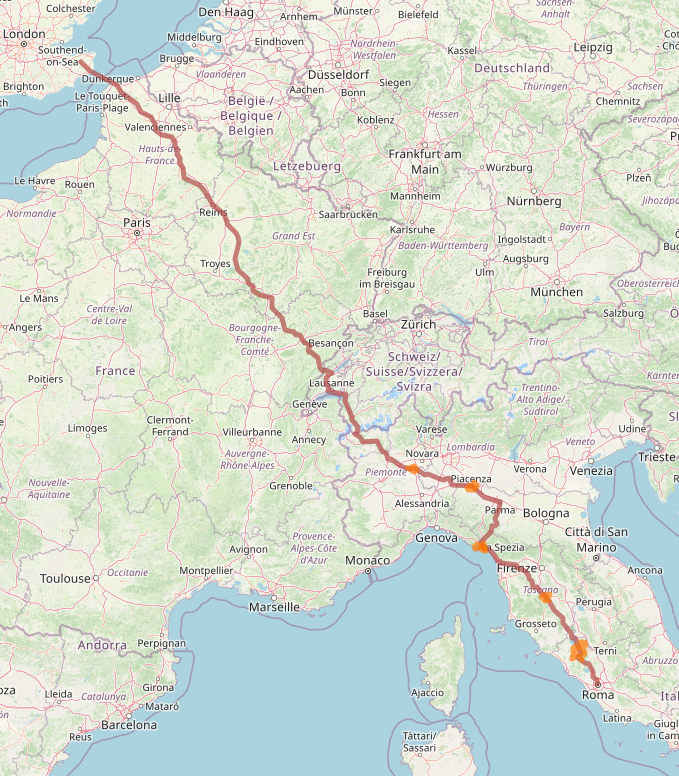
\includegraphics[scale=0.6]{img/francigena.png}}
    \caption{Visualization of Q6}
    \label{fig:francigena}
\end{figure}

\subsubsection*{Q7 - The places in Italy that are mentioned in works contained in manuscripts written in the fifteenth century }
In the following, we report the GeoSPARQL query corresponding to Q7. The results are displayed in \Cref{fig:italy}.

\begin{lstlisting}[caption=GeoSPARQL Query 7, label={lst:query7}]
PREFIX /*!\gls{xsd}!*/ <http://www.w3.org/2001/XMLSchema#>
PREFIX /*!\gls{rdf}!*/ <http://www.w3.org/1999/02/22-rdf-syntax-ns#>
PREFIX /*!\gls{rdfs}!*/ <http://www.w3.org/2000/01/rdf-schema#>
PREFIX /*!\gls{ecrm}!*/ <http://erlangen-crm.org/200717/>
PREFIX /*!\gls{ilrm}!*/ <http://imagoarchive.it/ilrmoo/>
PREFIX /*!\gls{imago}!*/ <https://imagoarchive.it/ontology/>
PREFIX /*!\gls{geo}!*/ <http://www.opengis.net/ont/geosparql#>
PREFIX /*!\gls{osm}!*/ <https://www.openstreetmap.org/>
PREFIX /*!\gls{osm2rdfkey}!*/ <https://osm2rdf.cs.uni-freiburg.de/rdf/key#>
PREFIX /*!\gls{geof}!*/ <http://www.opengis.net/def/function/geosparql/> 
PREFIX /*!\gls{wd}!*/ <http://www.wikidata.org/entity/>
SELECT DISTINCT ?authorName ?title ?toponymName ?wktPlace 
	FROM <https://geosparql.isti.cnr.it/fuseki/imago/archive>
		WHERE {
    ?exp_cre a ilrm:F28_Expression_Creation ;
  		     ilrm:R17_created ?work ;
         ecrm:P14_carried_out_by ?author ;
      		 ilrm:R18_created ?manuscript .
  ?author a imago:Author ;
          ecrm:P1_is_identified_by/ecrm:P190_has_symbolic_content ?authorName .
  ?work a ilrm:F2_Expression ;
        ecrm:P102_has_title/ecrm:P190_has_symbolic_content ?title ;
        ecrm:P106_is_composed_of ?toponym . 
  		?place imago:is_identified_by_toponym ?toponym ;
         		geo:asWKT ?wktPlace .
  		?toponym ecrm:P190_has_symbolic_content ?toponymName .
		?manifestation ilrm:R7i_is_materialized_in ?manuscript .
   		?manuscript ecrm:P1_is_identified_by/ecrm:P190_has_symbolic_content ?signature ;
		              ecrm:P50_has_current_keeper ?library ;
		              ecrm:P46_is_composed_of/ecrm:P1_is_identified_by/ecrm:P190_has_symbolic_content ?folios .
  		?library ecrm:P74_has_current_or_former_residence ?libraryPlace ;
		  			ecrm:P1_is_identified_by/ecrm:P190_has_symbolic_content ?libraryName .
  		?libraryPlace imago:is_identified_by_toponym ?top .
            ?top ecrm:P190_has_symbolic_content ?libraryPlaceName .
	  	?manifestation_creation ilrm:R24_created  ?manifestation ;
	 		        ecrm:P4_has_time-span/ecrm:P170i_time_is_defined_by ?date_manuscript ;
	    				:has_start_date ?start_date_manuscript ;
	 				:has_end_date ?end_date_manuscript .
		    FILTER("1401-01-01T00:00:00Z"^^xsd:dateTime <= ?start_date_manuscript && ?start_date_manuscript <= "1500-01-01T00:00:00Z"^^xsd:dateTime)
            FILTER("1401-01-01T00:00:00Z"^^xsd:dateTime <= ?end_date_manuscript && ?end_date_manuscript <= "1500-01-01T00:00:00Z"^^xsd:dateTime)
  BIND(CONCAT(?libraryPlaceName, ", ", ?libraryName, ", ",?signature, ", ", ?folios) AS ?manuscriptString)
  
  { 
    SELECT ?wktItaly 
    WHERE {
        SERVICE <https://qlever.cs.uni-freiburg.de/api/osm-planet> { 
            ?osm_id osm2rdfkey:wikidata wd:Q38 ;
                    a osm:relation ;
                    geo:hasGeometry ?geometryItaly .
            ?geometryItaly geo:asWKT ?wktItaly .     
        } 
    } LIMIT 1
  }
  FILTER(geof:sfWithin(?wktPlace,?wktItaly)). 
} 
\end{lstlisting}

% The query retrieves the toponyms and the corresponding works and authors in which these places are mentioned. In the WHERE clause, the polygons of the places identified by the toponyms are retrieved. Simultaneously, information regarding manuscripts is retrieved, including the production dates. Subsequently, the time range is established using the FILTER operator. A nested SELECT statement allows retrieving the WKT geometry of Italy (Q38) from the QLever \acrshort{SPARQLLabel} server of the University of Freiburg. Finally, another FILTER clause selects the places included within Italy's polygon.

The \Cref{lst:query7} retrieves distinct author names, work titles, place names, and WKT geometries of places associated with manuscripts created between 1401 and 1500, and stored in libraries within Italy.

Similar to query 5, there is a definition of prefixes and the \texttt{FROM} clause.

The \texttt{SELECT DISTINCT} statement (line 12) specifies:
\begin{itemize}
    \item \textit{authorName} - Author of the work.
    \item \textit{title} - Title of the work.
    \item \textit{toponymName} - Name of the place.
    \item \textit{wktPlace} - WKT representation of the place.
\end{itemize}

\textbf{WHERE Clause}
The \texttt{WHERE} block (lines 13-39) includes:
\begin{itemize}
    \item Patterns linking expression creation events, authors, works, and manuscripts.
    \item Retrieval of author and work details, including titles and toponyms.
    \item Information about manuscripts: signature, library, and folios.
    \item Library details, including residence and name.
    \item Time constraints for manuscript creation (1401-1500) using \texttt{FILTER} clauses.
\end{itemize}

\textbf{Nested SELECT Clause}
A nested \texttt{SELECT} block (lines 33-38) retrieves the WKT geometry of Italy:
\begin{itemize}
    \item Accesses the QLever endpoint to get Italy’s geometry from \acrshort{OSMLabel}.
    \item The \texttt{LIMIT 1} clause restricts to one result for faster retrieval.
\end{itemize}

\subsection*{Spatial Filter}
The \texttt{FILTER} clause (line 39) ensures that places are within Italy’s boundaries using \texttt{geof:sfWithin}.

\begin{figure}[h!tb]
    \centerline {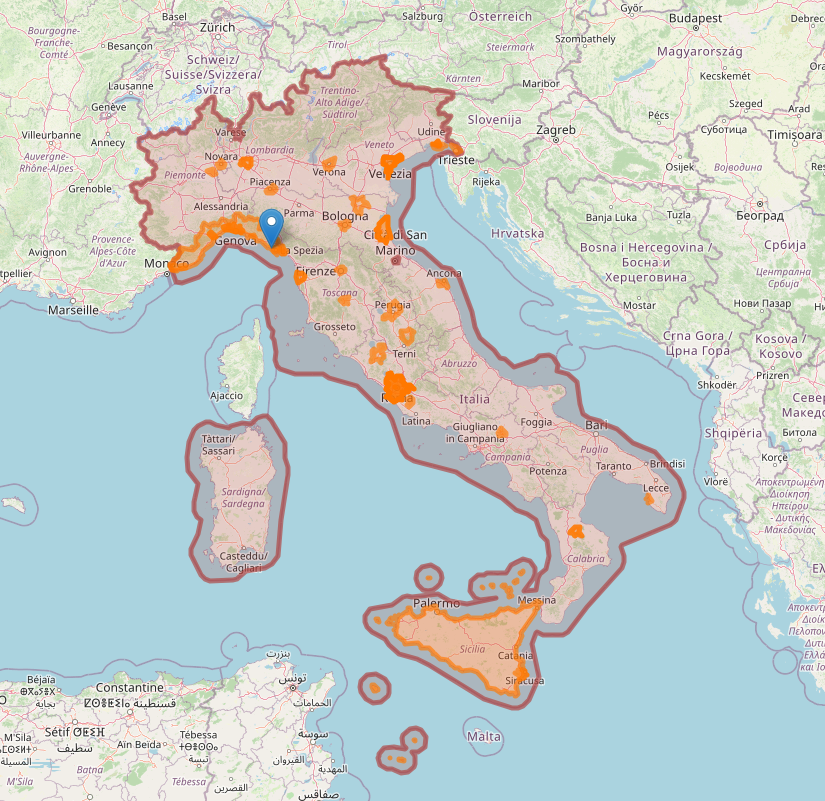
\includegraphics[scale=0.6]{img/italy.png}}
    \caption{Visualization of Q7}
    \label{fig:italy}
\end{figure}

\subsubsection{Q8 - The authors who have visited the Holy Land }
In the following, we report the GeoSPARQL query corresponding to Q8. The results are displayed in \Cref{tab:holyLand}.

\begin{lstlisting}[caption=GeoSPARQL Query 8, label={lst:query8}]
PREFIX /*!\gls{imago}!*/ <https://imagoarchive.it/ontology/>
PREFIX /*!\gls{igen}!*/ <https://imagoarchive.it/thes/tid/>
PREFIX /*!\gls{ecrm}!*/ <http://erlangen-crm.org/200717/>
PREFIX /*!\gls{ilrm}!*/ <http://imagoarchive.it/ilrmoo/>
PREFIX /*!\gls{wdt}!*/ <http://www.wikidata.org/prop/direct/>
PREFIX /*!\gls{wd}!*/ <http://www.wikidata.org/entity/>
PREFIX /*!\gls{geo}!*/ <http://www.opengis.net/ont/geosparql#>
PREFIX /*!\gls{geof}!*/ <http://www.opengis.net/def/function/geosparql/> 
PREFIX /*!\gls{uom}!*/ <http://www.opengis.net/def/uom/OGC/1.0/>

SELECT DISTINCT ?authorName ?title
FROM <https://geosparql.isti.cnr.it/fuseki/imago/archive>
WHERE {
  ?exp_cre a ilrm:F28_Expression_Creation ;
  		     ilrm:R17_created ?work ;
  		     ecrm:P14_carried_out_by ?author .	
  ?author a imago:Author ;
          ecrm:P1_is_identified_by/ecrm:P190_has_symbolic_content ?authorName .
  ?work a ilrm:F2_Expression ;
        ecrm:P102_has_title/ecrm:P190_has_symbolic_content ?title ;
        ecrm:P106_is_composed_of ?toponym . 
  ?place imago:is_identified_by_toponym ?toponym ;
         geo:asWKT ?wktPlace .
  ?toponym ecrm:P190_has_symbolic_content ?toponymName .
  
  ?work imago:has_genre igen:100026 . # Travel journal genre
  igen:100026  imago:has_genre_name ?labelGenre.
  
  { 
    SELECT ?coord 
    WHERE {
      SERVICE <https://query.wikidata.org/bigdata/namespace/wdq/sparql> { 
            wd:Q48175 wdt:P625 ?coord.    
      } 
    } LIMIT 1
  }
  FILTER(geof:sfIntersects(?wktPlace,geof:buffer(?coord,0.3, uom:degree))). 
}  
}  
\end{lstlisting}

% The query retrieves the authors who wrote works in which they tell their journeys in the Holy Land. In the WHERE clause the polygons of the places identified by the toponyms are retrieved only for the work belonging to the literary genre "personal travel diaries". As the Q2, this genre has a unique identifier (100026) that came from a literary genres thesaurus built by the IMAGO scholars. A nested SELECT statement allows retrieving the coordinates (longitude and latitude) of the Holy Land (Q48175) from the Wikidata SPARQL server. Finally, the FILTER clause selects the places that are included within a buffer of 0.3 degrees created around the Holy Land coordinates.

The \Cref{lst:query8} retrieves author names and titles of works belonging to the travel journal genre, filtered to include only those works associated with places intersecting a 0.3-degree buffer around a specific point.

Similar to query 5, there is a definition of prefixes and the \texttt{FROM} clause.

The \texttt{SELECT DISTINCT} statement (line 9) specifies:
\begin{itemize}
    \item \textit{authorName} - Author of the work.
    \item \textit{title} - Title of the work.
\end{itemize}

\textbf{WHERE Clause}
The main \texttt{WHERE} block (lines 10-24) defines the data retrieval conditions:
\begin{itemize}
    \item Links expression creation events, works, and authors.
    \item Retrieves author names, work titles, and place geometries in WKT format.
    \item Ensures the work belongs to the travel journal genre.
\end{itemize}

\textbf{Nested SELECT Clause}
A nested \texttt{SELECT} block (lines 18-23) retrieves coordinates from Wikidata:
\begin{itemize}
    \item Uses the Wikidata SPARQL endpoint to get the coordinates of Holy Land (wd:Q48175).
    \item The \texttt{LIMIT 1} clause restricts to one result for faster retrieval.
\end{itemize}

\textbf{Spatial Filter}
The \texttt{FILTER} clause (line 24) uses \texttt{geof:sfIntersects} to check if places intersect with a 0.3-degree buffer around the retrieved coordinates.

% The query produced the results reported in Figure \ref{fig:rivers}. All \acrshortpl{VCLabel} retrieved were correct and complete (Precision and Recall were 1). Therefore, the query was valuable in retrieving river-related \acrshortpl{VCLabel} and, by extension, could be used to extract water-basin-related \acrshortpl{VCLabel}.
\begin{table}[h!tb]
   \centering \caption{Result of the Query \ref{lst:query8}}
   \label{tab:holyLand}
   \vskip 0.2cm
   %%
   \scalebox{0.85}{
	    %% The {|c|c|c|c|c|} define the number of columns.
	    %% c means centered
	    %% | defines a vertical line between two columns 
	    \begin{tabular}{|c|c|c|}
	      \hline
	      # & authorName & title  \\
       \hline
1         & Guillelmus Gaudensis          & Peregrinationes totius Terrae Sanctae  \\
       \hline
2         & Felix Fabri                   & Evagatorium in Terrae sanctae, Arabiae et Egypti peregrinationem \\
       \hline 
3         & Ludovicus de Rupe Cavardi     & Itinerarium in Terram Sanctam   \\
\hline
4         & Iohannes de Mandavilla        & Itinerarius a terra Anglie in partes Iherosolomitanas et in ulteriores marinas \\
\hline
5         & Opus sine auctore             & Itinerarium cuiusdam Anglici Terram Sanctam et alia loca sancta visitantis \\
\hline
6         & Bernardus de Breydenbach      & Peregrinatio in Terram Sanctam \\
\hline
7         & Simeon Simeonis               & Itinerarium in Terram Sanctam \\
\hline
8         & Antonius de Reboldis          & Itinerarium ad Sepulcrum Domini  \\
\hline
9         & Opus sine auctore             & Narratio itineris navalis ad Terram Sanctam     \\
\hline
10        & Guilielmus de Boldensele      & Liber de quibusdam ultramarinis partibus et praecipue de Terra Sancta \\
\hline
11        & Bernardus monachus            & Itinerarium in loca sancta\\
\hline
12        & Opus sine auctore             & De itinere Frisonum   \\                              
\hline
13        & Paulus Waltherus de Guglingen & Itinerarium in Terram Sanctam et ad Sanctam Catharinam  \\    
\hline
14        & Wilbrandus Oldenburgensis     & Itinerarium Terrae Sanctae  \\
\hline
15        & Ludolphus de Sudheim          & De itinere Terrae Sanctae  \\            
\hline
16        & Anselmus Adurnus              & Itinerarium Terrae Sanctae  \\
\hline
	    \end{tabular}
	 }
 \end{table}


\subsection{An Example of Visualization: two Medieval Journeys as Story Maps}\label{VII-subsec:imago-visualization}

The SMBVT tool presented in \Cref{VII-subsec:moving-visualization} includes an additional visualization module that is better suited for creating and visualizing journeys or travel Story Maps. As defined, Story Maps visualize stories by embedding events within spatial contexts. The second module of SMBVT utilizes StoryMapJS \cite{knightlabStoryMapJS}, a JavaScript library for creating interactive map-based stories, which has been customized to fit the specific needs of SMBVT’s narrative visualization. By integrating this approach, the module provides another effective method for visualizing narratives, particularly those involving travel, thus expanding the scope of story representation. This technique directly contributes to addressing Research Question 3 (\ref{quote:rq3}), as it effectively employs spatial and narrative visualization to present complex information in an accessible and engaging manner.

Each event is connected to the preceding event by a dashed line, visually guiding users through the story’s temporal and spatial progression (see \Cref{fig:franceschino,fig:bruni}).

The main distinction from the other visualization is that events are pinned to specific geographic coordinates on the map, providing spatial context and guiding the user through the narrative in a sequence defined by the plot. Here, each story event is represented on the map as a distinct slide, containing essential information that enhances the storytelling experience.

StoryMapJS supports data represented as JSON. To align it with SMBVT’s visualization style, specific configurations were implemented, adapting the StoryMapJS JSON schema to meet SMBVT’s unique data requirements. This customization enabled direct mapping between the SMBVT PostgreSQL-JSON schema and the StoryMapJS JSON schema, facilitating seamless data transformation and visualization. The process of data integration from SMBVT to StoryMapJS involved precise schema mapping: SMBVT stores narrative data in a PostgreSQL-JSON schema, while StoryMapJS reads this data in a separate JSON format. This transformation converts event data, including geographic coordinates, media links, and descriptive text, from the SMBVT schema to the StoryMapJS format.

The Story Map structure still retains its division into two parts:
\begin{itemize}
    \item \textbf{Background Map:} Displayed on the left side, the background map visually anchors the story with geographic points marked by positional pins.
    \item \textbf{Event Information:} Displayed on the right side, containing detailed information about each event, including media objects and descriptive text.
\end{itemize}


\begin{figure}[h!tb]
    \centering
    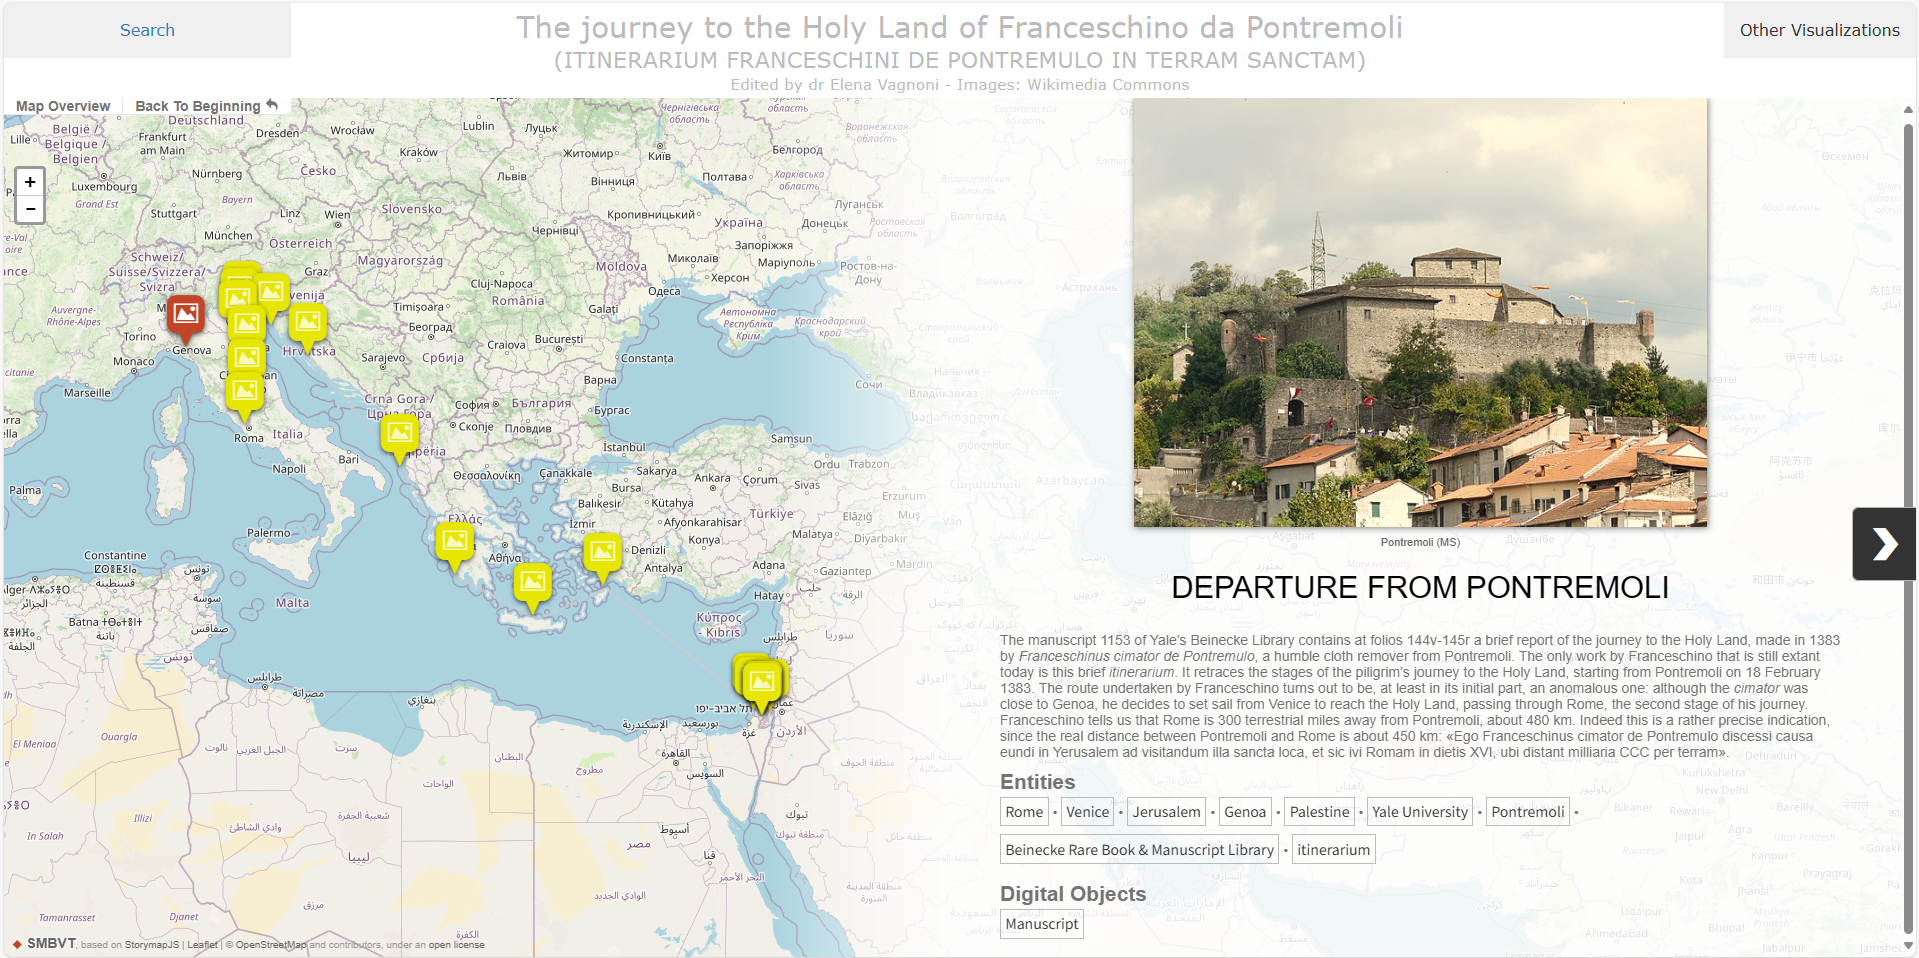
\includegraphics[scale=0.3]{img/franceschinoOverview.png}
    \caption{Overview of the Story Map "The Journey to the Holy Land of Franceschino da Pontremoli"}
    \label{fig:franceschino}
\end{figure}


This visualization technique aligns particularly well with the depiction of journeys or travels, as it effectively illustrates the trajectory of a journey by employing pins to denote key stages. A compelling historical instance of this approach is the pilgrimage to the Holy Land undertaken in 1383 by Franceschinus cimator de Pontremulo, a humble cloth remover from Pontremoli. The details of this pilgrimage are preserved in manuscript 1153 at Yale’s Beinecke Library, which documents the stages of Franceschino's pilgrimage, beginning in Pontremoli on February 18, 1383. The route taken by Franceschino is notable, particularly in its early phases, for its deviation from expected paths: despite the proximity of Pontremoli to Genoa, Franceschino chose to embark from Venice. This decision necessitated a detour through Rome, marking it as the second stage of his pilgrimage before proceeding to the Holy Land. The unique nature of Franceschino's path is vividly depicted in \Cref{fig:franceschino}, where each pin signifies a specific stage. By leveraging the story map, viewers can trace Franceschino’s journey interactively, gaining a narrative-driven exploration. Each stage is further enriched by contextual information, including associated participants, locations, and events. Such a graph structure can be queried to yield new insights, revealing connections otherwise obscured by the linear progression of text.


\begin{figure}[h!tb]
    \centering
    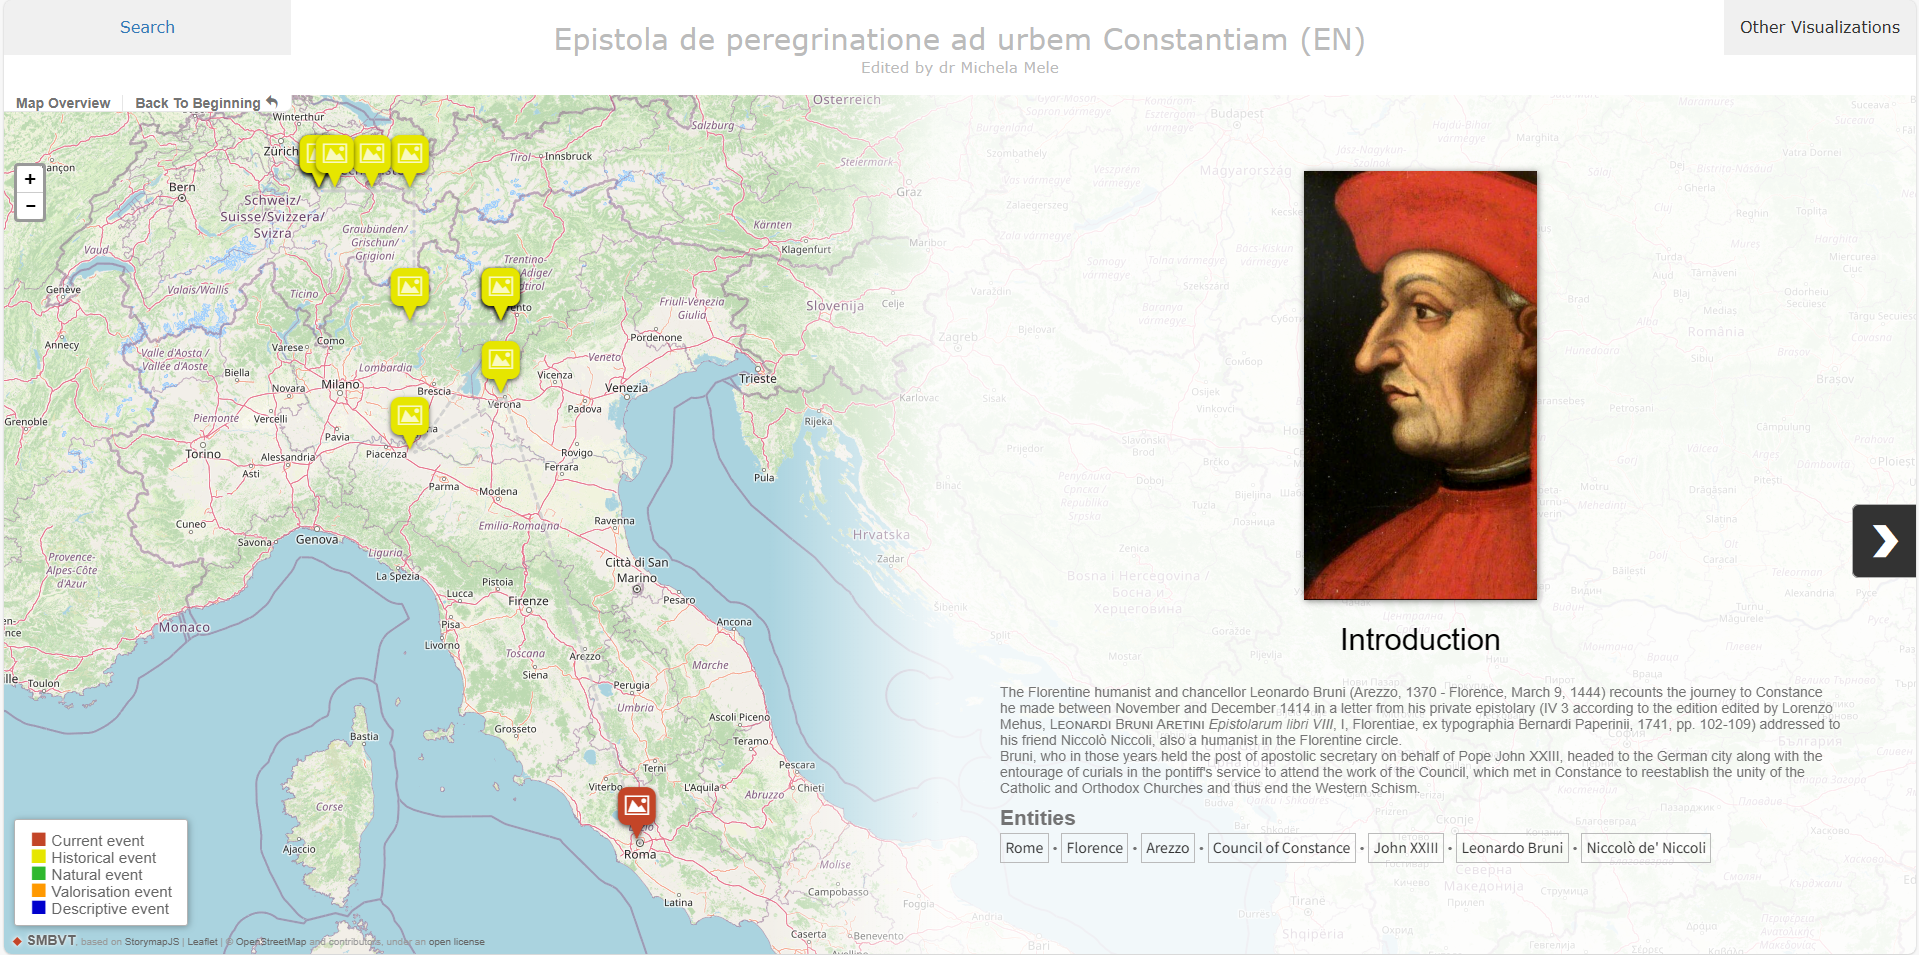
\includegraphics[scale=0.3]{img/bruniOverview.png}
    \caption{Overview of the Story Map "Epistola de peregrinatione ad urbem Constantiam"}
    \label{fig:bruni}
\end{figure}


In contrast, \Cref{fig:bruni} illustrates another significant journey: the voyage to Constance undertaken by the Florentine humanist and chancellor, Leonardo Bruni (1370–1444). Bruni recounts this journey, which occurred between November and December 1414, in a letter addressed to his friend Niccolò Niccoli, a fellow humanist within the Florentine intellectual circle. At the time, Bruni served as apostolic secretary to Pope John XXIII, travelling with the papal entourage to participate in the Council of Constance. This council aimed to reunify the Catholic and Orthodox Churches and bring an end to the Western Schism. Although Bruni's route is less immediately discernible compared to Franceschino's pilgrimage, the visual representation of the journey stages, marked as distinct events, remains highly informative. 

Employing SPARQL and GeoSPARQL queries on this knowledge graph offers a robust framework for discovering nuanced insights into Bruni's experiences. For instance, a notable anecdote emerges from Bruni’s fascination with the viticultural heritage of Termeno sulla Strada del Vino. As he travelled, he was struck by the region’s vineyards and the striking, the almost snowy appearance of the soil, which continues to yield the renowned white wine of Tramin, celebrated worldwide. This observation is not merely a historical curiosity; by integrating Bruni’s reflections with the \acrshort{MOVINGLabel} knowledge graph, one can draw connections across centuries, enriching our understanding of cultural and economic continuities within the winemaking tradition. The ability to query such structured information facilitates a multi-layered exploration, revealing insights that span both geographical and temporal dimensions.

\section{Discussion and Comparative Analysis}\label{VII-sec:discussion}

The interdisciplinary evaluation of NOnt+S, as applied to the \acrshort{MOVINGLabel} and \acrshort{IMAGOLabel} projects, provides critical insights into the ontology’s adaptability and effectiveness in modeling knowledge across varied, domain-specific contexts. This section offers a detailed exploration of NOnt+S’s performance, examining both its strengths and limitations in addressing the multifaceted needs of the bioeconomy and historical geography domains. The analysis not only emphasizes the ontology’s robustness in handling diverse semantic structures but also reflects on the broader implications for future applications in knowledge representation.

Within the \acrshort{MOVINGLabel} project, NOnt+S demonstrated remarkable proficiency in encapsulating the intricacies of bioeconomy and sustainability, particularly in mountain regions. The ontology’s flexible architecture facilitated the accurate representation of interconnected concepts such as agricultural practices, environmental conditions, and socio-economic dynamics. A major asset of NOnt+S was its capacity to integrate seamlessly with external geospatial datasets, including GISCO and \acrshort{OSMLabel}, thereby enhancing the granularity and accuracy of spatial data representations. This seamless integration allowed for comprehensive geospatial analysis, leveraging GeoSPARQL to perform sophisticated spatial queries. The modularity of the ontology proved to be instrumental in enriching domain-specific knowledge while maintaining compatibility with existing data standards. Nevertheless, the project also revealed areas where NOnt+S required further development. Specifically, the representation of specialized domains necessitated significant ontology customizations, which, while effective for the \acrshort{MOVINGLabel} project, introduced complexities that could hinder scalability and general applicability in broader or less uniform domains.

Turning to the \acrshort{IMAGOLabel} project, NOnt+S’s capacity to manage geospatial data within historical contexts emerged as a central strength. The ontology adeptly modeled place references derived from medieval texts, supporting in-depth analyses of geographic literature and the complex itineraries of medieval journeys. By leveraging external data repositories such as Wikidata and Pleiades, NOnt+S enriched historical geospatial information, demonstrating its versatility in addressing both temporal and spatial variability. However, the \acrshort{IMAGOLabel} project exposed unique challenges related to temporal alignment. Representing data across multiple, non-uniform historical periods required an intricate approach to ensure temporal consistency, complicating the ontology’s management of historical accuracy and logical coherence. The complexity of aligning medieval geographic concepts with modern data schemas imposed additional demands on data validation, requiring continuous monitoring to maintain semantic integrity.

Both projects utilized NOnt+S to facilitate the creation of structured knowledge graphs and enhance data visualization through Story Maps. These Story Maps were pivotal in narratively engaging users, weaving spatial references into a coherent visual exploration of medieval travel narratives. This method provided an intuitive interface for both academic researchers and the general public, making the historical data accessible and engaging. The success of Story Maps highlighted NOnt+S’s potential for transforming static historical and geographical data into dynamic, interactive experiences. Despite this, the projects also underscored the inherent complexity in ensuring uniform data integration when sourcing information from multiple, heterogeneous datasets. Addressing these complexities remains an area for future enhancement, suggesting that advancements in automated data alignment and refinement would be crucial for extending NOnt+S’s adaptability.

The comparative analysis of NOnt+S across the \acrshort{MOVINGLabel} and \acrshort{IMAGOLabel} projects illustrates the ontology’s significant potential for interdisciplinary applications, particularly in domains where narrative structures intersect with spatial data. Its adherence to Linked Open Data principles and standards-based design positions NOnt+S as a critical tool for facilitating cross-domain knowledge integration. Nevertheless, the ontology’s ability to scale and adapt to increasingly specialized and complex knowledge domains remains a challenge. To address these limitations, future iterations of NOnt+S may require refined support mechanisms for managing intricate extensions, improving semantic consistency, and optimizing automated data integration processes. Thus, while NOnt+S has proven its versatility and robustness, the evaluation also indicates pathways for further refinement, emphasizing the ontology’s continuous evolution to meet the demands of even more diverse and specialized research landscapes.

\subsection{Comparative Analysis of NOnt+S with Existing Ontologies and Representation Techniques}

The representation of narratives and their associated geospatial and temporal dimensions has emerged as a critical concern within knowledge modeling and digital humanities. In the previous Chapters we introduced the NOnt+S ontology, as an extension of the Narrative Ontology (NOnt), builds upon existing frameworks to address the challenges of integrating spatial semantics into narrative representation. Now we intend to introduce a thorough comparative analysis of NOnt+S against existing ontologies and knowledge representation approaches. Each comparison highlights the unique contributions of NOnt+S in addressing the limitations of earlier models.

The \Cref{table:comparative_analysis} summarizes the key features, strengths, and limitations of NOnt+S in comparison with existing ontologies and approaches.

\begin{table}[h!]\label{table:comparative_analysis}
\centering
\caption{Comparison of NOnt+S with Existing Ontologies and Techniques}
\label{tab:comparison}
 \scalebox{0.85}{
\begin{tabular}{|>{\raggedright}p{4cm}|>{\raggedright}p{4cm}|>{\raggedright}p{4cm}|>{\raggedright\arraybackslash}p{4cm}|}
\hline
\textbf{Ontology/Technique} & \textbf{Focus} & \textbf{Strengths} & \textbf{Limitations Overcome by NOnt+S} \\
\hline
CIDOC CRM & Event-based cultural heritage & Robust event and relationship modeling & Lacks explicit geospatial semantics and reasoning capabilities. \\
\hline
Narrative Cartography & Visual storytelling through maps & Spatio-temporal visualization of narratives & Static; lacks computational reasoning and semantic formalization. \\
\hline
InTaVia & Post-anthropocentric storytelling & Supports multiple narrative entities and visualization & No formal reasoning; lacks geospatial querying and semantic interoperability. \\
\hline
Ciotti's Formal Ontology & Narrative components: characters, traits, and spaces & Formal OWL-based representation of narrative semantics & Focused on textual abstraction; lacks spatial semantics and reasoning. \\
\hline
% \textbf{NOnt+S} & Narrative, geospatial, and temporal representation & Integrates geospatial semantics, formal reasoning, and advanced querying & Combines strengths of other approaches while addressing their limitations. \\
% \hline
\end{tabular}
}
\end{table}

As discussed in \Cref{III-subsec:cidoccrm}, the CIDOC CRM serves as a widely endorsed framework for modeling cultural heritage data, emphasizing the temporal and relational dynamics between entities. Its robust ontology provides a solid foundation for organizing historical and event-based knowledge, effectively supporting the mapping of cultural narratives. However, while CRM excels in modeling event-centric relationships, its capacity to capture the nuanced spatial semantics critical for geospatial narratives remains limited. The CRMgeo extension addresses this limitation by incorporating geospatial data modeling capabilities, yet it falls short of comprehensively representing narratives with detailed spatial semantics and reasoning capabilities. NOnt+S emerges as a solution to this challenge by extending the capabilities of CRM to explicitly integrate narrative structures and geospatial reasoning. Utilizing GeoSPARQL and OWL 2 DL, NOnt+S formalizes both qualitative and quantitative spatial relationships, enabling them to be computationally analyzed and reasoned upon. By embedding geospatial concepts such as proximity, topological relationships, and distances within a narrative framework, NOnt+S bridges the gap left by CRMgeo, facilitating a richer and more dynamic approach to geospatial narratives that supports advanced querying and inferential processes.

Narrative cartography, as conceptualized by scholars such as Caquard and Cartwright\cite{caquardNarrativeCartographyMapping2014}, highlights the interplay between spatial representation and storytelling, focusing on how maps can encapsulate the temporal, emotional, and ambiguous aspects of narratives. Traditional cartographic approaches, however, often rely on static visualizations and manually integrated spatial data, limiting their potential for computational analysis. NOnt+S revolutionizes narrative cartography by embedding it within a formal semantic framework, transforming static maps into dynamic, machine-readable representations. This approach enables the encoding of spatial and narrative data in formats that support automated reasoning and querying, uncovering hidden patterns and relationships within geospatial narratives. Through the use of OWL 2 DL, NOnt+S enables sophisticated inferential capabilities, which allow researchers to move beyond visualization and into deeper analytical understanding. By formalizing the spatial semantics of narratives, NOnt+S transcends the limitations of conventional narrative cartography, offering tools to dynamically explore and infer the complexities of geospatial storytelling.

Interactive platforms like InTaVia \cite{kusnickEveryThingCan2024} represent a significant innovation in the domain of cultural heritage and digital humanities by integrating visualization, data retrieval, and storytelling into cohesive, user-friendly interfaces. These platforms excel in constructing dynamic narratives that incorporate diverse entities, such as individuals, artifacts, locations, and institutions, and challenge anthropocentric biases by foregrounding the roles of non-human actors. Through interactive visualizations, InTaVia fosters an immersive user experience, enabling the exploration of complex relationships within cultural narratives. However, while platforms like InTaVia are highly effective at visualizing and integrating heterogeneous data, they lack the formal reasoning mechanisms required for deeper computational analysis. NOnt+S addresses this gap by embedding narratives within a semantically rich framework, integrating geospatial semantics with OWL 2 DL and GeoSPARQL to enable advanced reasoning and querying capabilities. This approach not only complements the visualization strengths of platforms like InTaVia but also facilitates a more profound analytical understanding of spatial narratives, bridging the divide between interactive visualization and formal computational analysis.

Fabio Ciotti's formal ontology for narrative \cite{ciottiFormalOntologyNarrative2016} represents a significant contribution to computational narratology, drawing upon semiotic and structuralist traditions to conceptualize narrative elements in machine-readable formats. Building on the theories of scholars like Greimas and Lotman, Ciotti formalizes key narrative components, including characters, traits, and spaces, using OWL 2 to represent these constructs systematically. His ontology emphasizes the dual roles of characters as actors and functional entities, inspired by Greimas' actantial model, allowing for the systematic analysis of their actions, traits, and relationships within a narrative structure. Additionally, Ciotti integrates Lotman's concept of semiotic space to model the interactions between characters and their narrative environments, offering a robust framework for textual analysis. Despite its innovative approach, Ciotti's ontology remains focused on abstract narrative structures, with limited engagement in geospatial reasoning. NOnt+S builds on Ciotti's conceptual foundation by incorporating the spatial and temporal dimensions of narratives, leveraging GeoSPARQL and OWL 2 DL to enable advanced geospatial querying and reasoning. This integration enhances the narrative framework by aligning textual semantics with spatial analytics, providing a comprehensive platform for analyzing, visualizing, and reasoning about complex geospatial narratives. In doing so, NOnt+S not only extends the analytical depth of formal ontologies but also positions itself as a pioneering tool for bridging narrative semantics and geospatial representation.


NOnt+S advances the state of narrative modeling by combining semantic reasoning, geospatial querying, and narrative formalization into a unified framework. Unlike earlier approaches, such as CIDOC CRM, knowledge graphs, and narrative cartography, NOnt+S explicitly integrates spatial semantics, ensuring that geospatial relationships can be formally represented and reasoned upon. While platforms like InTaVia prioritize visualization and interaction, NOnt+S provides the formal structure necessary for computational querying and inference. By incorporating spatial semantics, NOnt+S builds upon Fabio Ciotti's formal ontology, extending its narrative modeling capabilities into the geospatial domain. This ontology sets a new standard for narrative knowledge representation, bridging the gap between visualization, reasoning, and semantic interoperability.

\subsection{Adapting the NOnt+S Framework to Other Domains}

The NOnt+S framework demonstrates significant potential for adaptation across a range of domains, leveraging its strengths in semantic modeling, modular design, and querying capabilities. By addressing domain-specific challenges while maintaining general applicability, NOnt+S can be extended to meet the demands of diverse research and application areas. Below, we present a detailed exploration of considerations and enhancements required for such adaptations.
The modular architecture of NOnt+S, which has already proven effective in domains such as bioeconomy and geographic literature, can be generalized to suit broader applications. This requires separating foundational modules for semantic modeling, encompassing temporal, spatial, and narrative elements, from domain-specific extensions. Such a separation ensures that the core ontology remains reusable and flexible, while domain adapters or plugins can interface with specialized vocabularies and taxonomies. For instance, in the healthcare domain, NOnt+S could incorporate clinical narratives, such as patient journeys and treatment pathways, while linking geospatial data to public health studies, maybe with the integration of established biomedical ontologies.
Linking NOnt+S to domain-specific and open knowledge bases is essential for enriched data representation in areas such as urban planning or climate science. This integration involves using specialized datasets, such as Urban Atlas for urban planning or IPCC reports for climate change, and employing dynamic linking mechanisms. Automated enrichment processes can map NOnt+S entities to resources like GeoNames or domain-specific extensions of Wikidata, enabling seamless access to comprehensive and authoritative information. Such enhancements ensure that NOnt+S can support intricate narratives while maintaining alignment with evolving knowledge repositories.
While NOnt+S already supports advanced querying via GeoSPARQL and SPARQL, certain domains may require additional enhancements. Historical and archaeological applications, for example, demand temporal reasoning to model and query ancient events and their progression over time. Similarly, domains like environmental science or economics could benefit from causal and probabilistic reasoning to analyze relationships within complex datasets. These extensions would allow NOnt+S to address sophisticated research questions, expanding its analytical scope and utility.
Different domains exhibit unique user interaction requirements, necessitating customizable interfaces for the NOnt+S framework. In healthcare, visual dashboards can track real-time patient data and enable predictive modeling. Education could benefit from interactive story maps to support curriculum design, while social sciences might require tools for visualizing social networks and relationships. By incorporating user-centric design principles, NOnt+S can enhance accessibility and usability, fostering adoption across diverse fields.
Certain domains, such as cultural heritage preservation or biomedicine, necessitate careful attention to ethical and cultural factors. Incorporating modules for ethical reasoning, such as those ensuring compliance with data privacy and consent requirements, is essential. Similarly, the framework should adapt ontological representations to account for cultural variations, particularly in global projects. These considerations enhance the relevance and sensitivity of NOnt+S in diverse sociocultural contexts.
The flexibility of NOnt+S opens opportunities for applications in emerging domains. In artificial intelligence ethics, the framework could model decision-making narratives to ensure transparency and accountability. For space exploration, NOnt+S can represent interplanetary missions, facilitating reasoning about extraterrestrial geospatial data. Additionally, the gaming and entertainment industry could utilize NOnt+S to structure interactive narratives for virtual environments, offering innovative solutions for immersive storytelling.


\section{Conclusion}\label{VII-sec:conclusion}

The interdisciplinary evaluation of the NOnt+S ontology across bioeconomy studies and geographic literature has demonstrated its effectiveness in modeling domain-specific knowledge while maintaining flexibility and extensibility. Through its modular structure, NOnt+S was able to accommodate diverse concepts, ranging from resource management in the bioeconomy to spatial relations in geographic literature.

The application of the framework presented in the \textit{Framework} chapter has further validated NOnt+S as a robust ontology for interdisciplinary research. Future work will focus on addressing the identified challenges, particularly concerning the integration of highly specialized concepts and ensuring consistent data validation across even broader domains.


